\documentclass[compsoc,draftclsnofoot,onecolumn,10pt]{IEEEtran}
\usepackage[utf8]{inputenc}
\usepackage{color}
\usepackage{url}

\usepackage{pdfpages}

\usepackage{graphicx}

\usepackage{enumitem}

\usepackage[letterpaper, margin=.75in]{geometry}

\usepackage{hyperref}
\usepackage{listings}

\usepackage[dvipsnames]{xcolor}
\usepackage{pgfgantt}

\definecolor{dkgreen}{rgb}{0,0.6,0}
\definecolor{gray}{rgb}{0.5,0.5,0.5}
\definecolor{mauve}{rgb}{0.58,0,0.82}

\renewcommand{\lstlistingname}{Code Example} % a listing caption title.

\lstset{
	frame=single,
	language=C,
	columns=flexible,
	numbers=left,
	numbersep=5pt,
	numberstyle=\tiny\color{gray},
	keywordstyle=\color{blue},
	commentstyle=\color{dkgreen},
	stringstyle=\color{mauve},
	breaklines=true,
	breakatwhitespace=true,
	tabsize=4,
	captionpos=b
}

\def\name{Cierra Shawe, Daniel Stoyer, Tao Chen}

%% The following metadata will show up in the PDF properties
\hypersetup{
	colorlinks = false,
	urlcolor = black,
	pdfauthor = {\name},
	pdfkeywords = {Final Report, Winter 2017},
	pdftitle = {Final Report},
	pdfsubject = {Final Report for ARC},
	pdfpagemode = UseNone
}

\def\myversion{1.0}
\date{}
%
%\usepackage{titlesec}
%
%\usepackage{hyperref}

\parindent = 0.0 in
\parskip = 0.1 in

% \title{Capstone Final Report}
% \author{Dan Stoyer, Cierra Shawe, Tao Chen }
% \date{June 2017}

\begin{document}
\begin{titlepage}
	\title{Final Report\\
	ARC - Autonomous RC}
	\author{Tao Chen, Cierra Shawe, Daniel Stoyer}
	\maketitle
	\begin{center}
		\today
	\end{center}

	\thispagestyle{empty} % gets rid of the "0" page number.
	
\end{titlepage}

\tableofcontents

\newpage

\section{Introduction}
Research into consumer/hobbyist, high performance RC vehicles was requested by Oregon State University via Mr. Kevin McGrath. This project was requested to determine if it is possible to apply high-speed performance during autonomous navigation and obstacle avoidance to a modified RC car at a cost less than four thousand dollars (USD). Autonomous RC (ARC) sought to push the boundaries of what is possible for autonomous RC vehicles. Our research shows that components are decreasing in cost and increasing in performance. The cost-barrier to autonomous research is decreasing dramatically. Our documentation and parts list provides would-be researchers a launching point to continue the work we started in ARC. Our client was the same person who requested the project, Mr. Kevin McGrath. Mr. McGrath is an instructor at Oregon State University. [Who are the members of our team?]The ARC team members are Tao Chen, Cierra Shawe, and Daniel Stoyer. [What were their roles?]Tao was our software and robotics expert, he worked extensively with our software package and got our car working in simulation, he was responsible for the areas of Motion Model, Path Planning, and Autonomous Algorithms (e.g. obstacle avoidance, parallel parking, etc.). Cierra was our electronics and hardware expert, she designed all the mounting hardware used to anchor the sensors to the RC car and did all the wiring/soldering, she was responsible for the ares of Vision Systems, Sensors, and Hardware. Dan was team leader, responsible for making sure the team was on track to hit milestones and Capstone deadlines on time. He was also responsible for overseeing the areas of Image Analysis, User Interfaces, and Radio Communication. [What was the role of the client? (i.e. supervision only, participate in development, etc.)]
\newpage
\section{Original Requirements Document}

% SRS document goes here.

\includepdf[pages=1-17]{orig_srs_document}

    \subsection{Requirements Changes}
    No major or minor changes were made to the requirements document. We found that our initial assessment was accurate throughout the project and our client agreed.
    % Table for Client changes go here.
    % \section{Document Revision History}
\begin{table}[h]
\resizebox{\textwidth}{!}{\begin{tabular}{ p{2cm}|p{1cm}|p{3cm}|p{3cm}|p{3cm}|  }

\multicolumn{5}{c}{Version History} \label{history}\\
\cline{2-2}
\multicolumn{1}{c|}{ } & Version & \multicolumn{1}{c}{ } & \multicolumn{1}{c}{ } & \multicolumn{1}{c}{ } \\
% Column format:
%<col1>&<col2>&<col3>&<col4>
%& Version & & \\
\hline
\multicolumn{1}{|c|}{Team Member}& & Cierra & Tao & Dan \\
\hline
 & v1.0 & {\tiny Initial version.} & {\tiny Initial version.} & {\tiny Initial version.} \\
\cline{2-5}
% empty first column | Cierra's changes | Tao's Changes | Dan's changes
 & v1.1 &
 % Cierra's changes
 {\tiny
 \begin{itemize}
 	\item Cierra's change \#1
 	\item Cierra's change \#2
 	\item ...
 \end{itemize}
 }
 &
 % Tao's changes
 {\tiny
  \begin{itemize}
 	\item Tao's change \#1
 	\item Tao's change \#2
 	\item ...
 \end{itemize}
 }
 &
 % Dan's changes
 {\tiny
  \begin{itemize}
 	\item Updated gantt chart with progress from Fall and Winter terms.
 \end{itemize}
 }

 \\ % End of v1.1 changes
\cline{2-5}

\end{tabular}}
\end{table}

% Final gantt chart goes here.

%%%%%%%%%% How to use these Gantt Charts %%%%%%%%%%
%%% IMPORTANT!!! %%%
% Within the \ganttchart[]{} code, ONLY adjust dates
%
% Each Gantt chart has an area preceding it to adjust values.
%
% When adding a group or task, use the existing code in the SRS section as a 
% template.
%
% The overall progress for a group is tracked by getting the average of all the 
% subtasks. So, if you add a subtask, be sure to add the count variable to the
% overall average computation and increase the denominator by one
% Example progress average:
%
% \newcount\srsprogress
% \srsprogress=\the\numexpr(
% 	  \introprog 
% 	+ \overalldescprog 
% 	+ \specificreqprog 
% 	+ \othernonfunreqprog 
% 	+ \otherreqprog
% 	+ \indexprog 
% 	+ \appendixprog
% 	)/7 % divided by number of subtasks
%%%%%%%%%%%%%%%%%%%%%%%%%%%%%%%%%%%%%%%%%%%%%%%%%%%


%%%%% Fall Term Chart Oct 14 - Dec. 09 %%%%%%%

%%%%%%%%%%%%%%%%%%%%%%%%%%%%%%%%%%%%%%%%%%%%%%%%%%%
% Set progress and dates for groups and tasks here.
%%%% Term Date Range %%%%
\newcommand{\fallstart}{2016-10-14}
\newcommand{\fallend}{2016-12-09}

%%%% SRS (Due: Oct 28) %%%%

%Introduction
\newcount\introprog
\introprog=100

% Overall Description
\newcount\overalldescprog
\overalldescprog=100

% Specific Requirements
\newcount\specificreqprog
\specificreqprog=100

% Other Non-Functional Requirements
\newcount\othernonfunreqprog
\othernonfunreqprog=100

% Other Requirements
\newcount\otherreqprog
\otherreqprog=100

% Index
\newcount\indexprog
\indexprog=100

% Apppendix
\newcount\appendixprog
\appendixprog=100

% Overall SRS progress

% NOTE
\newcount\srsprogress
\srsprogress=\the\numexpr(
  \introprog 
+ \overalldescprog 
+ \specificreqprog 
+ \othernonfunreqprog 
+ \otherreqprog
+ \indexprog 
+ \appendixprog
)/7
%%%%%%%%%%%%%%%%%%%%%%

%%%% Technology Review (Due: Nov. 04) %%%%
\newcount\techprogress
\techprogress=100
%%%%%%%%%%%%%%%%%%%%%%

%%%% Design Document (Due: Nov. 23) %%%%
\newcount\designprogress
\designprogress=100
%%%%%%%%%%%%%%%%%%%%%%

%%%% Fall Progress Report (Due: Dec. 09) %%%%
\newcount\fprogress
\fprogress=100
%%%%%%%%%%%%%%%%%%%%%%

%%%%%%%%%%%%%%%%%%%%%%%%%%%%%%%%%%%%%%%%%%%%%%%%%
\begin{figure}[h]
	\caption{ARC Fall Schedule Gantt Chart}	
	\begin{ganttchart}[
		y unit title=0.4cm,
		y unit chart=0.5cm,
		x unit=0.2665cm,
		vgrid,
		%	time slot format=isodate-yearmonth,
		time slot format=isodate,
		%	compress calendar,
		title/.append style={fill=RoyalBlue!50!black},
		title label font=\sffamily\bfseries\color{white},
		title label node/.append style={below=-1.6ex},
		title left shift=.05,
		title right shift=-.05,
		title height=1,
		bar/.append style={draw=none, fill=OliveGreen!75},
		bar height=.6,
		bar label font=\normalsize\color{RawSienna},
		group/.append style={draw=none, fill=MidnightBlue},
		group incomplete/.append style={fill=YellowOrange},
		group right shift=0,
		group top shift=.6,
		group height=.3,
		group peaks height=.2,
		bar incomplete/.append style={fill=Maroon}
		]{\fallstart}{\fallend}
		
		\ganttset{
			calendar week text={
				\pgfcalendarmonthshortname{\startmonth}~\startday
			}
		}
		\gantttitle{Fall 2016}{57}\\
		\gantttitlecalendar{week} \\
		\ganttset{progress label text={}, link/.style={black!63, -to}}
		
		%%%% SRS (Due: Oct 28) %%%%
		\ganttgroup[progress={\srsprogress}]{Requirements Document}{2016-10-14}{2016-10-28} \\
		\ganttbar[progress={\introprog}]{Introduction}{2016-10-14}{2016-10-28} \\
		\ganttbar[progress={\overalldescprog}]{Overall Description}{2016-10-14}{2016-10-28} \\
		\ganttbar[progress={\specificreqprog}]{Specific Requirements}{2016-10-14}{2016-10-28} \\
		\ganttbar[progress={\othernonfunreqprog}]{Other Non-Functional Req.}{2016-10-14}{2016-10-28} \\
		\ganttbar[progress={\otherreqprog}]{Other Req.}{2016-10-14}{2016-10-28} \\
		\ganttbar[progress={\indexprog}]{Index}{2016-10-14}{2016-10-28} \\
		\ganttbar[progress={\appendixprog}]{Appendix}{2016-10-14}{2016-10-28} \\
		
		
		%%%% Technology Review (Due: Nov. 04) %%%%
		\ganttgroup[progress={\techprogress}]{Tech Review}{2016-10-29}{2016-11-04} \\
		
		%%%% Design Document (Due: Nov. 23) %%%%
		\ganttgroup[progress={\designprogress}]{Design Doc}{2016-11-05}{2016-11-23} \\
		
		%%%% Fall Progress Report (Due: Dec. 09) %%%%
		\ganttgroup[progress={\fprogress}]{Fall Report}{2016-11-24}{2016-12-09} \\
		
		%	\ganttset{link/.style={OliveGreen}}
	\end{ganttchart}
\end{figure}

%%%%% Winter Term Chart JAN 09 - MAR 24 %%%%%

%%%%%%%%%%%%%%%%%%%%%%%%%%%%%%%%%%%%%%%%%%%%%%%%%%%
%%%% Term Date Range %%%%
\newcommand{\winterstart}{2017-01-09}
\newcommand{\winterend}{2017-03-24}

% Set progress and dates for groups and tasks here.

%%%% Alpha level release (with demo) (Due: Feb. 24, 2017) %%%%
\newcount\alphaprogress
\alphaprogress=75

%%%% Beta level release (with demo) (Due: Mar. 24, 2017) %%%%
\newcount\betaprogress
\betaprogress=0

%%%% Winter progress report (Due: Mar. 24, 2017) %%%%
\newcount\wprogress
\wprogress=0
%
%
%
%
%%%%%%%%%%%%%%%%%%%%%%%%%%%%%%%%%%%%%%%%%%%%%%%%%%%
\begin{figure}[h]
	\caption{ARC Winter Schedule Gantt Chart}
	\begin{ganttchart}[
		y unit title=0.4cm,
		y unit chart=0.5cm,
		x unit=0.227cm,
		vgrid,
		%	time slot format=isodate-yearmonth,
		time slot format=isodate,
		%	compress calendar,
		title/.append style={draw=none, fill=RoyalBlue!50!black},
		title label font=\sffamily\bfseries\color{white},
		title label node/.append style={below=-1.6ex},
		title left shift=.05,
		title right shift=-.05,
		title height=1,
		bar/.append style={draw=none, fill=OliveGreen!75},
		bar height=.6,
		bar label font=\normalsize\color{RawSienna},
		group/.append style={draw=none, fill=MidnightBlue},
		group incomplete/.append style={fill=YellowOrange},
		group right shift=0,
		group top shift=.6,
		group height=.3,
		group peaks height=.2,
		bar incomplete/.append style={fill=Maroon}
		]{\winterstart}{\winterend}
		
		\ganttset{
			calendar week text={
				\pgfcalendarmonthshortname{\startmonth}~\startday
			}
		}
		\gantttitle{Winter 2017}{75}\\
		\gantttitlecalendar{week} \\
		\ganttset{progress label text={}, link/.style={black!63, -to}}
		
		%%%% Alpha level release (with demo) (Due: Feb. 24, 2017) %%%%
		\ganttgroup[progress={\alphaprogress}]{Alpha Release}{2017-01-09}{2017-02-24} \\
		
		%%%% Beta level release (with demo) (Due: Mar. 24, 2017) %%%%
		\ganttgroup[progress={\betaprogress}]{Beta Release}{2017-02-25}{2017-03-24} \\
		
		%%%% Winter progress report (Due: Mar. 24, 2017) %%%%
		\ganttgroup[progress={\wprogress}]{Winter Report}{2017-02-25}{2017-03-24} \\
		
		%	\ganttset{link/.style={OliveGreen}}
	\end{ganttchart}
\end{figure}

%%%%%% End Winter Term %%%%%

%%%%%% Spring Term Chart APR 3 - JUN 16 %%%%%

%%%%%%%%%%%%%%%%%%%%%%%%%%%%%%%%%%%%%%%%%%%%%%%%%%%%%%%
%%%% Term Date Range %%%%
\newcommand{\springstart}{2017-04-03}
\newcommand{\springend}{2017-06-16}
%	% Set progress and dates for groups and tasks here.


%%%% 1.0 level release (Due: May 15, 2017) %%%%
\newcount\releaseprogress
\releaseprogress=0

%%%% Engineering Expo (Due: May 19) %%%%
\newcount\expoprogress
\expoprogress=0

%%%% Final Report (Due: June 16) %%%%
\newcount\finalrepprogress
\finalrepprogress=0
%
%
%
%%%%%%%%%%%%%%%%%%%%%%%%%%%%%%%%%%%%%%%%%%%%%%%%%%%%%%%
\begin{figure}[h]
	\caption{ARC Spring Schedule Gantt Chart}	
	\begin{ganttchart}[
		y unit title=0.4cm,
		y unit chart=0.5cm,
		x unit=0.231cm,
		vgrid,
		%	time slot format=isodate-yearmonth,
		time slot format=isodate,
		%	compress calendar,
		title/.append style={draw=none, fill=RoyalBlue!50!black},
		title label font=\sffamily\bfseries\color{white},
		title label node/.append style={below=-1.6ex},
		title left shift=.05,
		title right shift=-.05,
		title height=1,
		bar/.append style={draw=none, fill=OliveGreen!75},
		bar height=.6,
		bar label font=\normalsize\color{RawSienna},
		group/.append style={draw=none, fill=MidnightBlue},
		group incomplete/.append style={fill=YellowOrange},
		group right shift=0,
		group top shift=.6,
		group height=.3,
		group peaks height=.2,
		bar incomplete/.append style={fill=Maroon}
		]{\springstart}{\springend}
		
		\ganttset{
			calendar week text={
				\pgfcalendarmonthshortname{\startmonth}~\startday
			}
		}
		\gantttitle{Spring 2017}{75}\\
		\gantttitlecalendar{week} \\
		\ganttset{progress label text={}, link/.style={black!63, -to}}
		
		%%%% 1.0 level release (Due: May 15, 2017) %%%%
		\ganttgroup[progress={\releaseprogress}]{1.0 Release}{2017-04-03}{2017-05-15} \\
		
		%%%% Engineering Expo (Due: May 19) %%%%
		\ganttgroup[progress={\expoprogress}]{Spring Expo}{2017-05-16}{2017-05-19} \\
		
		%%%% Winter progress report (Due: Mar. 24, 2017) %%%%
		\ganttgroup[progress={\finalrepprogress}]{Final Report}{2017-05-20}{2017-06-16} \\
		
		%	\ganttset{link/.style={OliveGreen}}
	\end{ganttchart}
\end{figure}

%%%%%% End Spring Term %%%%%


\section{Design Document}
    \subsection{Original Design Document}
    % original design document here.

\includepdf[pages=1-12]{orig_arc_design_document}
    
    \subsection{Changes in Design}
    We had to make several changes to our design throughout the life of the project. We moved away from stereo vision for obstacle avoidance and went with lidar instead. This had a cascading effect on other parts of our design. Since we didn't use stereo vision, our image analysis design also changed. We didn't need to worry about communicating images over the network so our communication protocols became much more simple.
    

\section{Tech Review}
    \subsection{Original Tech Review Document}
    % original tech review document goes here.
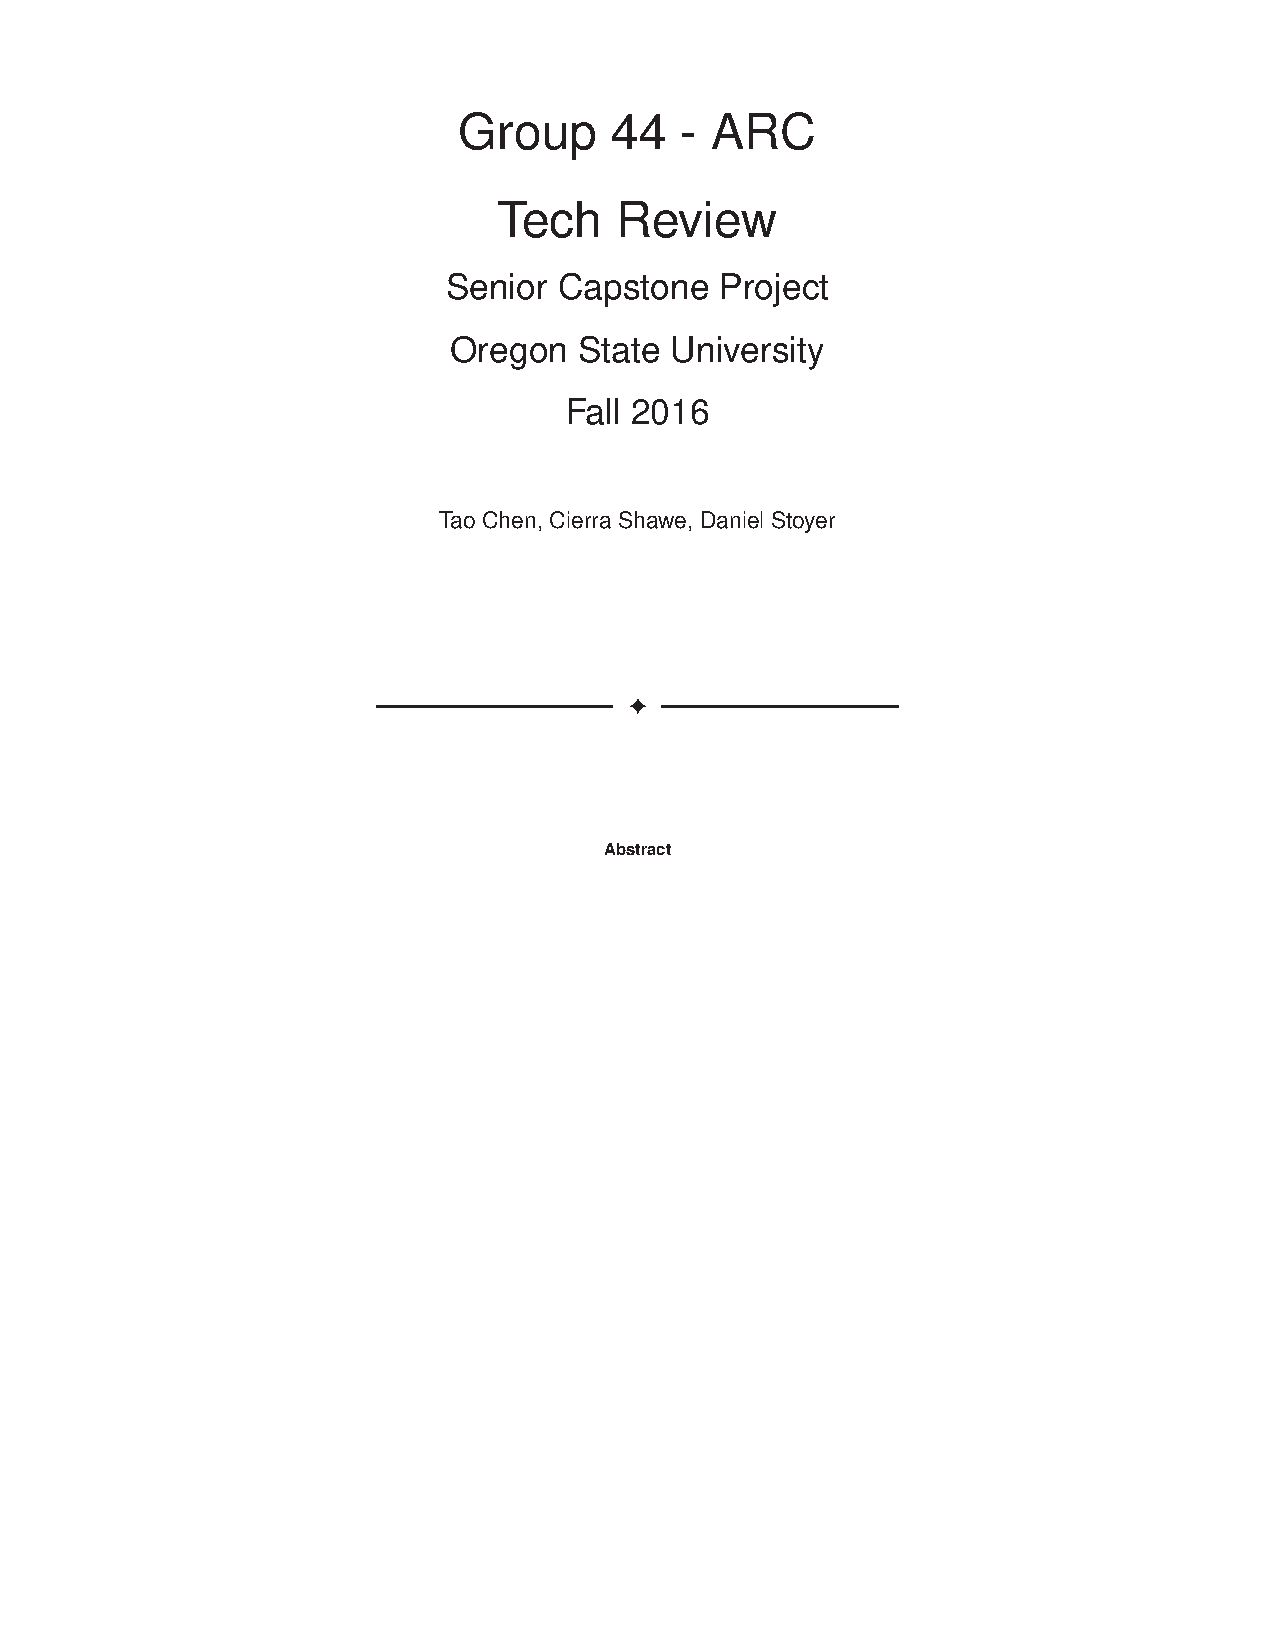
\includepdf[pages=1-12]{orig_tech_review}

    \subsection{Changes in Tech}
    As our research and development process matured, we discovered different ways of doing things and changed direction on some of the technology we used for the project. We changed from stereo vision to lidar for depth-finding and obstacle detection. We changed from using the PXFMini autopilot with the Raspberry Pi 3 to using a PWM controller with an Arduino to control motors and servos. We want to use the Q Ground Control GUI to control the vehicle remotely, but had to scratch that when we abandoned the PXFMini. We switched to using RVIZ (visualization package for ROS) for vehicle control


\section{Weekly Blogs}

\subsection{Cierra's Blog Entries}

\subsubsection{Fall Week 4}
\begin{itemize}
    \item {\textbf{Worked On}}
    \begin{itemize}

    \end{itemize}

    \item {\textbf{Problems Encountered}}
    \begin{itemize}

    \end{itemize}

    \item{\textbf{Plans for next week}}
    \begin{itemize}

    \end{itemize}

\end{itemize}

\subsubsection{Fall Week 5}
\begin{itemize}
    \item {\textbf{Worked On}}
    \begin{itemize}

    \end{itemize}

    \item {\textbf{Problems Encountered}}
    \begin{itemize}

    \end{itemize}

    \item{\textbf{Plans for next week}}
    \begin{itemize}

    \end{itemize}

\end{itemize}

\subsubsection{Fall Week 6}
\begin{itemize}
    \item {\textbf{Worked On}}
    \begin{itemize}

    \end{itemize}

    \item {\textbf{Problems Encountered}}
    \begin{itemize}

    \end{itemize}

    \item{\textbf{Plans for next week}}
    \begin{itemize}

    \end{itemize}

\end{itemize}

\subsubsection{Fall Week 7}
\begin{itemize}
    \item {\textbf{Worked On}}
    \begin{itemize}

    \end{itemize}

    \item {\textbf{Problems Encountered}}
    \begin{itemize}

    \end{itemize}

    \item{\textbf{Plans for next week}}
    \begin{itemize}

    \end{itemize}

\end{itemize}

\subsubsection{Fall Week 8}
\begin{itemize}
    \item {\textbf{Worked On}}
    \begin{itemize}

    \end{itemize}

    \item {\textbf{Problems Encountered}}
    \begin{itemize}

    \end{itemize}

    \item{\textbf{Plans for next week}}
    \begin{itemize}

    \end{itemize}

\end{itemize}

\subsubsection{Fall Week 9}
\begin{itemize}
    \item {\textbf{Worked On}}
    \begin{itemize}

    \end{itemize}

    \item {\textbf{Problems Encountered}}
    \begin{itemize}

    \end{itemize}

    \item{\textbf{Plans for next week}}
    \begin{itemize}

    \end{itemize}

\end{itemize}

\subsubsection{Fall Week 10}
\begin{itemize}
    \item {\textbf{Worked On}}
    \begin{itemize}

    \end{itemize}

    \item {\textbf{Problems Encountered}}
    \begin{itemize}

    \end{itemize}

    \item{\textbf{Plans for next week}}
    \begin{itemize}

    \end{itemize}

\end{itemize}

\subsubsection{Fall Week 11}
\begin{itemize}
    \item {\textbf{Worked On}}
    \begin{itemize}

    \end{itemize}

    \item {\textbf{Problems Encountered}}
    \begin{itemize}

    \end{itemize}

    \item{\textbf{Plans for next week}}
    \begin{itemize}

    \end{itemize}

\end{itemize}

\subsubsection{Winter Week 1}
\begin{itemize}
    \item {\textbf{Worked On}}
    \begin{itemize}

    \end{itemize}

    \item {\textbf{Problems Encountered}}
    \begin{itemize}

    \end{itemize}

    \item{\textbf{Plans for next week}}
    \begin{itemize}

    \end{itemize}

\end{itemize}

\subsubsection{Winter Week 2}
\begin{itemize}
    \item {\textbf{Worked On}}
    \begin{itemize}

    \end{itemize}

    \item {\textbf{Problems Encountered}}
    \begin{itemize}

    \end{itemize}

    \item{\textbf{Plans for next week}}
    \begin{itemize}

    \end{itemize}

\end{itemize}

\subsubsection{Winter Week 3}
\begin{itemize}
    \item {\textbf{Worked On}}
    \begin{itemize}

    \end{itemize}

    \item {\textbf{Problems Encountered}}
    \begin{itemize}

    \end{itemize}

    \item{\textbf{Plans for next week}}
    \begin{itemize}

    \end{itemize}

\end{itemize}

\subsubsection{Winter Week 4}
\begin{itemize}
    \item {\textbf{Worked On}}
    \begin{itemize}

    \end{itemize}

    \item {\textbf{Problems Encountered}}
    \begin{itemize}

    \end{itemize}

    \item{\textbf{Plans for next week}}
    \begin{itemize}

    \end{itemize}

\end{itemize}

\subsubsection{Winter Week 5}
\begin{itemize}
    \item {\textbf{Worked On}}
    \begin{itemize}

    \end{itemize}

    \item {\textbf{Problems Encountered}}
    \begin{itemize}

    \end{itemize}

    \item{\textbf{Plans for next week}}
    \begin{itemize}

    \end{itemize}

\end{itemize}

\subsubsection{Winter Week 6}
\begin{itemize}
    \item {\textbf{Worked On}}
    \begin{itemize}

    \end{itemize}

    \item {\textbf{Problems Encountered}}
    \begin{itemize}

    \end{itemize}

    \item{\textbf{Plans for next week}}
    \begin{itemize}

    \end{itemize}

\end{itemize}

\subsubsection{Winter Week 7}
\begin{itemize}
    \item {\textbf{Worked On}}
    \begin{itemize}

    \end{itemize}

    \item {\textbf{Problems Encountered}}
    \begin{itemize}

    \end{itemize}

    \item{\textbf{Plans for next week}}
    \begin{itemize}

    \end{itemize}

\end{itemize}

\subsubsection{Winter Week 8}
\begin{itemize}
    \item {\textbf{Worked On}}
    \begin{itemize}

    \end{itemize}

    \item {\textbf{Problems Encountered}}
    \begin{itemize}

    \end{itemize}

    \item{\textbf{Plans for next week}}
    \begin{itemize}

    \end{itemize}

\end{itemize}

\subsubsection{Winter Week 9}
\begin{itemize}
    \item {\textbf{Worked On}}
    \begin{itemize}

    \end{itemize}

    \item {\textbf{Problems Encountered}}
    \begin{itemize}

    \end{itemize}

    \item{\textbf{Plans for next week}}
    \begin{itemize}

    \end{itemize}

\end{itemize}

\subsubsection{Winter Week 10}
\begin{itemize}
    \item {\textbf{Worked On}}
    \begin{itemize}

    \end{itemize}

    \item {\textbf{Problems Encountered}}
    \begin{itemize}

    \end{itemize}

    \item{\textbf{Plans for next week}}
    \begin{itemize}

    \end{itemize}

\end{itemize}

\subsubsection{Winter Week 11}
\begin{itemize}
    \item {\textbf{Worked On}}
    \begin{itemize}

    \end{itemize}

    \item {\textbf{Problems Encountered}}
    \begin{itemize}

    \end{itemize}

    \item{\textbf{Plans for next week}}
    \begin{itemize}

    \end{itemize}

\end{itemize}

\subsubsection{Spring Week 1}
\begin{itemize}
    \item {\textbf{Worked On}}
    \begin{itemize}

    \end{itemize}

    \item {\textbf{Problems Encountered}}
    \begin{itemize}

    \end{itemize}

    \item{\textbf{Plans for next week}}
    \begin{itemize}

    \end{itemize}

\end{itemize}

\subsubsection{Spring Week 2}
\begin{itemize}
    \item {\textbf{Worked On}}
    \begin{itemize}

    \end{itemize}

    \item {\textbf{Problems Encountered}}
    \begin{itemize}

    \end{itemize}

    \item{\textbf{Plans for next week}}
    \begin{itemize}

    \end{itemize}

\end{itemize}

\subsubsection{Spring Week 3}
\begin{itemize}
    \item {\textbf{Worked On}}
    \begin{itemize}

    \end{itemize}

    \item {\textbf{Problems Encountered}}
    \begin{itemize}

    \end{itemize}

    \item{\textbf{Plans for next week}}
    \begin{itemize}

    \end{itemize}

\end{itemize}

\subsubsection{Spring Week 4}
\begin{itemize}
    \item {\textbf{Worked On}}
    \begin{itemize}

    \end{itemize}

    \item {\textbf{Problems Encountered}}
    \begin{itemize}

    \end{itemize}

    \item{\textbf{Plans for next week}}
    \begin{itemize}

    \end{itemize}

\end{itemize}

\subsubsection{Spring Week 5}
\begin{itemize}
    \item {\textbf{Worked On}}
    \begin{itemize}

    \end{itemize}

    \item {\textbf{Problems Encountered}}
    \begin{itemize}

    \end{itemize}

    \item{\textbf{Plans for next week}}
    \begin{itemize}

    \end{itemize}

\end{itemize}

\subsubsection{Spring Week 6}
\begin{itemize}
    \item {\textbf{Worked On}}
    \begin{itemize}

    \end{itemize}

    \item {\textbf{Problems Encountered}}
    \begin{itemize}

    \end{itemize}

    \item{\textbf{Plans for next week}}
    \begin{itemize}

    \end{itemize}

\end{itemize}

\subsubsection{Spring Week 7}
\begin{itemize}
    \item {\textbf{Worked On}}
    \begin{itemize}

    \end{itemize}

    \item {\textbf{Problems Encountered}}
    \begin{itemize}

    \end{itemize}

    \item{\textbf{Plans for next week}}
    \begin{itemize}

    \end{itemize}

\end{itemize}

\subsubsection{Spring Week 8}
\begin{itemize}
    \item {\textbf{Worked On}}
    \begin{itemize}

    \end{itemize}

    \item {\textbf{Problems Encountered}}
    \begin{itemize}

    \end{itemize}

    \item{\textbf{Plans for next week}}
    \begin{itemize}

    \end{itemize}

\end{itemize}

\subsection{Tao's Blog Entries}

\subsubsection{Fall Week 4}
\begin{itemize}
    \item {\textbf{Worked On}}
    \begin{itemize}
      \item Worked on the problem statement performance measure section.
    \end{itemize}

    \item {\textbf{Problems Encountered}}
    \begin{itemize}
      \item None.
    \end{itemize}

    \item{\textbf{Plans for next week}}
    \begin{itemize}
      \item None.
    \end{itemize}

\end{itemize}

\subsubsection{Fall Week 5}
\begin{itemize}
    \item {\textbf{Worked On}}
    \begin{itemize}
      \item Have not contributed so far.
    \end{itemize}

    \item {\textbf{Problems Encountered}}
    \begin{itemize}
      \item None.
    \end{itemize}

    \item{\textbf{Plans for next week}}
    \begin{itemize}
      \item None.
    \end{itemize}

\end{itemize}

\subsubsection{Fall Week 6}
\begin{itemize}
    \item {\textbf{Worked On}}
    \begin{itemize}
      \item The SRS document.
    \end{itemize}

    \item {\textbf{New}}
    \begin{itemize}
      \item Have a better and clear view of the project.
      \item An abstract block diagram that depicts the structure of the project.
    \end{itemize}

    \item {\textbf{Problems Encountered}}
    \begin{itemize}
      \item Still a lot of unclear/unspecified aspects of the project.
    \end{itemize}

    \item{\textbf{Plans for next week}}
    \begin{itemize}
      \item Individual writing.
    \end{itemize}

\end{itemize}

\subsubsection{Fall Week 7}
\begin{itemize}
    \item {\textbf{Worked On}}
    \begin{itemize}
      \item SRS document.
      \item Tasks breakdown list.
    \end{itemize}

    \item {\textbf{Problems Encountered}}
    \begin{itemize}
      \item Still a lot of uncertainties on what hardware/interface we are using.
    \end{itemize}

    \item{\textbf{Plans for next week}}
    \begin{itemize}
      \item Finish SRS document.
      \item Finish tech review.
    \end{itemize}

\end{itemize}

\subsubsection{Fall Week 8}
\begin{itemize}
    \item {\textbf{Worked On}}
    \begin{itemize}
      \item Worked on the SRS document and the Tech Review. Did research on
      efficiency of specific algorithms. Since our vehicle will eventually
      run in different environments, possibly not predefined, algorithms
      must be robust as well. Thought about the project as a whole. Realized
      that we could only have a more and more thorough understanding of the
      different aspects of this project.
    \end{itemize}

    \item {\textbf{Problems Encountered}}
    \begin{itemize}
      \item We still need more hardware. The SRS document hasn't been
      finished yet. The research we are doing currently may turn out to be
      in the wrong direction.
    \end{itemize}

    \item{\textbf{Plans for next week}}
    \begin{itemize}
      \item Tech review and the SRS document.
    \end{itemize}

\end{itemize}

\subsubsection{Fall Week 9}
\begin{itemize}
    \item {\textbf{Worked On}}
    \begin{itemize}
      \item Tech review and the SRS document.
    \end{itemize}

    \item {\textbf{Problems Encountered}}
    \begin{itemize}
      \item Haven't started the design document yet.
    \end{itemize}

    \item{\textbf{Plans for next week}}
    \begin{itemize}
      \item Start the design doc ASAP. Get more hardware in hand.
      \item We'd better have a clear view (graph/list) of we need
      to accomplish along with potential solutions.
    \end{itemize}

\end{itemize}

\subsubsection{Fall Week 10}
\begin{itemize}
    \item {\textbf{Worked On}}
    \begin{itemize}
      \item None.
    \end{itemize}

    \item {\textbf{Problems Encountered}}
    \begin{itemize}
      \item None.
    \end{itemize}

    \item{\textbf{Plans for next week}}
    \begin{itemize}
      \item None.
    \end{itemize}

\end{itemize}

\subsubsection{Fall Week 11}
\begin{itemize}
    \item {\textbf{Worked On}}
    \begin{itemize}
      \item None.
    \end{itemize}

    \item {\textbf{Problems Encountered}}
    \begin{itemize}
      \item None.
    \end{itemize}

    \item{\textbf{Plans for next week}}
    \begin{itemize}
      \item None.
    \end{itemize}

\end{itemize}

\subsubsection{Winter Week 1}
\begin{itemize}
    \item {\textbf{Worked On}}
    \begin{itemize}
      \item Ros on the NUC is fully functional.
      \item Tested the Lidar unit. It worked great.
      \item Went through some tutorials on Ros.
    \end{itemize}

    \item {\textbf{Some thoughts on the project}}
    \begin{itemize}
      \item Start our development on the NUC and see if it is possible to
      migrate all functionalities to the Intel board at the end.
      \item Start with the Lidar to implement obstacle avoidance.
      \item The two cameras we were given provide two separate feeds. I
      think we need two video streams in one feed such that we only need to
      dedicate one port to it and it will provide a better interface to
      interact with the images.
      \item Need to mount the two cameras on something rigid.
    \end{itemize}

\end{itemize}

\subsubsection{Winter Week 2}
\begin{itemize}
    \item {\textbf{Worked On}}
    \begin{itemize}
      \item Ros tutorials.
    \end{itemize}

    \item {\textbf{Problems Encountered}}
    \begin{itemize}
      \item A lot of software only supports certain versions of Ros.
    \end{itemize}

    \item{\textbf{Plans for next week}}
    \begin{itemize}
      \item Car model on Gazebo.
    \end{itemize}

\end{itemize}

\subsubsection{Winter Week 3}
\begin{itemize}
    \item {\textbf{Worked On}}
    \begin{itemize}
      \item More Ros tutorials. RC car model on Gazebo. Simple shape with a
      rectangular box as the chassis and four wheels.
    \end{itemize}

    \item {\textbf{Problems Encountered}}
    \begin{itemize}
      \item Ros Indigo only works with Gazebo 2.X, which doesn't have the
      model editor built-in. So we have to code our URDF file.
    \end{itemize}

    \item{\textbf{Plans for next week}}
    \begin{itemize}
      \item Finish the RC car model over the weekend. Make it move in
      Gazebo. Add sensors to it.
    \end{itemize}

\end{itemize}

\subsubsection{Winter Week 4}
\begin{itemize}
    \item {\textbf{Worked On}}
    \begin{itemize}
      \item Modified the AutoRally car model.
      \item Added a lidar unit and a camera unit to the model.
      \item Retrieved data from the two sensors and display
      results in real time in Gazebo successfully in simulation.
      \item Migrated part of the AutoRally codes to our own package.
      \item Tried to figure out the dependencies between nodes/packages
      within the AutoRally project so that we can reuse some of them.
      \item Working on a documentation as well.
    \end{itemize}

    \item {\textbf{Problems Encountered}}
    \begin{itemize}
      \item AutoRally is a huge project and there is a lot of physics
      involved. It might take a little bit longer than expected to go
      through all the nodes/package.
      \item The lidar unit worked flawlessly in Gazebo. However, the point
      cloud produced by the camera unit was rotated 90 degrees up. Worked
      on it for one day, trying to rotate it so that it actually reflects
      the reality. No luck.
    \end{itemize}

    \item{\textbf{Plans for next week}}
    \begin{itemize}
      \item Keep on working on migrating codes. Plan to finish it by the end
      of this week. And then we can add our own stuff to it.
      \item Try to get the car moving in the simulation.
    \end{itemize}

\end{itemize}

\subsubsection{Winter Week 5}
\begin{itemize}
    \item {\textbf{Worked On}}
    \begin{itemize}
      \item No entry.
    \end{itemize}

    \item {\textbf{Problems Encountered}}
    \begin{itemize}
      \item No entry.
    \end{itemize}

    \item{\textbf{Plans for next week}}
    \begin{itemize}
      \item No entry.
    \end{itemize}

\end{itemize}

\subsubsection{Winter Week 6}
\begin{itemize}
    \item {\textbf{Worked On}}
    \begin{itemize}
      \item No entry.
    \end{itemize}

    \item {\textbf{Problems Encountered}}
    \begin{itemize}
      \item No entry.
    \end{itemize}

    \item{\textbf{Plans for next week}}
    \begin{itemize}
      \item No entry.
    \end{itemize}

\end{itemize}

\subsubsection{Winter Week 7}
\begin{itemize}
    \item {\textbf{Worked On}}
    \begin{itemize}
      \item No entry.
    \end{itemize}

    \item {\textbf{Problems Encountered}}
    \begin{itemize}
      \item No entry.
    \end{itemize}

    \item{\textbf{Plans for next week}}
    \begin{itemize}
      \item No entry.
    \end{itemize}

\end{itemize}

\subsubsection{Winter Week 8}
\begin{itemize}
    \item {\textbf{Worked On}}
    \begin{itemize}
      \item No entry.
    \end{itemize}

    \item {\textbf{Problems Encountered}}
    \begin{itemize}
      \item No entry.
    \end{itemize}

    \item{\textbf{Plans for next week}}
    \begin{itemize}
      \item No entry.
    \end{itemize}

\end{itemize}

\subsubsection{Winter Week 9}
\begin{itemize}
    \item {\textbf{Worked On}}
    \begin{itemize}
      \item No entry.
    \end{itemize}

    \item {\textbf{Problems Encountered}}
    \begin{itemize}
      \item No entry.
    \end{itemize}

    \item{\textbf{Plans for next week}}
    \begin{itemize}
      \item No entry.
    \end{itemize}

\end{itemize}

\subsubsection{Winter Week 10}
\begin{itemize}
    \item {\textbf{Worked On}}
    \begin{itemize}
      \item No entry.
    \end{itemize}

    \item {\textbf{Problems Encountered}}
    \begin{itemize}
      \item No entry.
    \end{itemize}

    \item{\textbf{Plans for next week}}
    \begin{itemize}
      \item No entry.
    \end{itemize}

\end{itemize}

\subsubsection{Winter Week 11}
\begin{itemize}
    \item {\textbf{Worked On}}
    \begin{itemize}
      \item No entry.
    \end{itemize}

    \item {\textbf{Problems Encountered}}
    \begin{itemize}
      \item No entry.
    \end{itemize}

    \item{\textbf{Plans for next week}}
    \begin{itemize}
      \item No entry.
    \end{itemize}

\end{itemize}

Note:\par
None indicates no blog posts were made for those weeks.\par
No entry means blogs and notes were made but did not get posted and will
appear on later blog posts.

\subsubsection{Spring Week 1}
\begin{itemize}
    \item {\textbf{Worked On}}
    \begin{itemize}
      \item In the last two weeks of winter term I didn't do the whole lot
      mainly because of finals. However, I managed to get the car to follow
      paths. It turned the path planning algorithm didn't generate paths for
      the car to follow. Instead, it generates commands to drive to car. That
      made things very easy. All I did was translate the commands for the
      controller. So that's done. I have decided to use the teb\_local\_planner
      as our path planning package. I integrated it into the smart\_driving
      package and set it to work on car-like robot. According to the ros wiki
      for the car-like setup, the configuration is only experimental. Just
      something to keep in mind. It may sometimes output unpredictable behaviors.
      Since the teb\_local\_planner also does obstacle avoidance, obstacle
      avoidance was handled.
    \end{itemize}

    \item {\textbf{Problems Encountered}}
    \begin{itemize}
      \item The steering commands oscillate a lot. The oscillation makes the
      movements of the car unnatural. We need to look deeper into the code
      to make sure the steering is smooth.
      \item Obstacle avoidance requires a lot of computing power. It requires
      so much that it's undoable on this laptop. The algorithm does obstacle
      avoidance by computing the costmap each time it sees a new objects.
      (detected by laser scans) A costmap is basically a 2D grid that describes
      the environment and helps to calculate the most efficient path. On this
      computer, a new costmap takes on average 3 seconds to compute. When
      there's no objects, the algorithm works fine on this computer. Note that
      the costmap is only updated when objects are detected. Not sure if the
      NUC can handle it. Need to find out.
      \item The software can be simplified. When I have been doing is just
      adding new nodes. I didn't consider if the nodes are actually necessary.
      It's because I didn't want to spend time on going over the AutoRally
      packages. For example, when I need to translate some data, I just make
      a node to do the task. In fact, I could have just remap the message
      name in the launch file. That will reduce a lot of overhead. It will
      possibly make the software run faster. I will make a table to figure
      out the data flow and delete all unnecessary nodes.
    \end{itemize}

    \item{\textbf{Plans for next week}}
    \begin{itemize}
      \item Continue working on the navigation.
    \end{itemize}

\end{itemize}

\subsubsection{Spring Week 2}
\begin{itemize}
    \item {\textbf{Worked On}}
    \begin{itemize}
      \item We decided to move away from AutoRally a little bit because it was
      too complicated. We tried ROS stage, which was a 2D simulation platform.
      It's simpler than Gazebo. We quickly got the teb\_local\_planning working
      because we already had it working with AutoRally.
    \end{itemize}

    \item {\textbf{Problems Encountered}}
    \begin{itemize}
      \item I am not sure if stage can simulate gps and imu. It will only simulate
      laser scan right now. If we couldn't get the imu and gps simulated on
      stage, it is fine. We can do it directly on the car.
    \end{itemize}

    \item{\textbf{Plans for next week}}
    \begin{itemize}
      \item Get the imu and gps working.
    \end{itemize}

\end{itemize}

\subsubsection{Spring Week 3}
\begin{itemize}
    \item {\textbf{Worked On}}
    \begin{itemize}
      \item Got the odometry in Stage working.
      \item Worked on the poster.
    \end{itemize}

    \item {\textbf{Problems Encountered}}
    \begin{itemize}
      \item Stage doesn't simulate IMU.
    \end{itemize}

    \item{\textbf{Plans for next week}}
    \begin{itemize}
      \item Keep working on Stage and the poster.
    \end{itemize}

\end{itemize}

\subsubsection{Spring Week 4}
\begin{itemize}
    \item {\textbf{Worked On}}
    \begin{itemize}
      \item Didn't do a whole lot because I was at a point where if I couldn't
      get the imu data I couldn't move forward in integrating the navigation
      stack. Dan and I were working on it. But we didn't make much progress.
      I had a lot homework to do. So I left it to Dan. Looks like he hasn't
      gotten it working yet.
    \end{itemize}

    \item {\textbf{Problems Encountered}}
    \begin{itemize}
      \item The IMU driver provided by ROS outputs imu data. However, the state
      estimator receives a constant pointer to the data. We need to find a way to
      transmit the data.
    \end{itemize}

    \item{\textbf{Plans for next week}}
    \begin{itemize}
      \item Keep working on the IMU. If that's done. Move on to the GPS.
    \end{itemize}

\end{itemize}

\subsubsection{Spring Week 5}
\begin{itemize}
    \item {\textbf{Worked On}}
    \begin{itemize}
      \item Worked on the GPS. The data from the GPS was not reliable.
      \item Looked for other options for state estimation, because we
      couldn't the way around the constant pointer.
      \item Found one package that seemed promising.
    \end{itemize}

    \item {\textbf{Problems Encountered}}
    \begin{itemize}
      \item The AutoRally state estimator was a perfect package to use. But
      we didn't have the right hardware. The new package we found was intuitive
      but had a lot of parameters that needed to set up.
      \item We are still not able to set it up.
    \end{itemize}

    \item{\textbf{Plans for next week}}
    \begin{itemize}
      \item Keep trying the new package.
      \item Start preparing for Expo (demo).
    \end{itemize}

\end{itemize}

\subsubsection{Spring Week 6}
\begin{itemize}
    \item {\textbf{Worked On}}
    \begin{itemize}
      \item Midterm progress report.
      \item IMU and GPS.
      \item Code Freeze. Documentation.
      \item Simulation.
    \end{itemize}

    \item {\textbf{Problems Encountered}}
    \begin{itemize}
      \item Our software is very environment-dependent, meaning that it might not
      be able to run on another computer if the environment was not set up right.
      \item GPS data was still not reliable. Can't just work with the IMU.
      \item We might need wheel encoders.
    \end{itemize}

    \item{\textbf{Plans for next week}}
    \begin{itemize}
      \item Keep preparing for the expo.
      \item Keep experimenting the new package.
    \end{itemize}

\end{itemize}

\subsubsection{Spring Week 7}
\begin{itemize}
    \item {\textbf{Worked On}}
    \begin{itemize}
      \item Prepared the system for expo demo.
      \item Expo pitch.
      \item Expo.
    \end{itemize}

    \item {\textbf{Problems Encountered}}
    \begin{itemize}
      \item A lot of software was installed on the laptop.
      \item Wasn't able to run the leddar during Expo, which was kind
      of embarrassing.
    \end{itemize}

    \item{\textbf{Plans for next week}}
    \begin{itemize}
      \item Relax.
      \item Relax more.
      \item Relax even more.
      \item Relax a little bit more.
      \item Then start working on the final write up.
    \end{itemize}

\end{itemize}

\subsubsection{Spring Week 8}
\begin{itemize}
    \item {\textbf{If you were to redo the project from Fall term, what would you tell yourself?}}
    \begin{itemize}
      \item I would tell myself that my team would win the first prize at the end of the year.
      \item I would tell myself to get as many sensors as possible.
      \item I would tell myself this project was one of the coolest projects so do your best.
    \end{itemize}

    \item {\textbf{What's the biggest skill you've learned?}}
    \begin{itemize}
      \item Using ROS.
      \item Communication.
    \end{itemize}

    \item{\textbf{What skills do you see yourself using in the future?}}
    \begin{itemize}
      \item Since I will be doing robotics, I think knowing how to use ROS will greatly benefit me.
      \item I want to do research or development, which means I will most likely be working in a
      team. Good communication skill will also benefit me lot.
    \end{itemize}

    \item{\textbf{What did you like about the project, and what did you not?}}
    \begin{itemize}
      \item I like everything about this project.
      \item I don't like the fact that we were given so many writing assignments.
    \end{itemize}

    \item{\textbf{What did you learn from your teammates?}}
    \begin{itemize}
      \item I think my understanding of sarcasm improves a little bit.
      \item Most importantly, it's collaboration. I was working in a team with more
      than 15 people. I didn't really learn a lot from that team. A three person team
      is a good starting point. We can distribute the work load evenly and still have
      a complete picture of the project.
    \end{itemize}

    \item{\textbf{If you were the client for this project, would you be satisfied with the work done?}}
    \begin{itemize}
      \item I will be satisfied but a little disappointed because the car can't drive itself.
    \end{itemize}

    \item{\textbf{If your project were to be continued next year, what do you think needs to be working on?}}
    \begin{itemize}
      \item To make the project a little easier, I think we need to get another car first,
      or make one ourselves. We didn't have much information about the car we have right
      now. and that car is too much for our purposes. I want the wheels to be completely
      rigid or just with thin tires. I don't want the car to have less complicated
      suspensions and drive train.
      \item With a new customized car, we can add wheel encoders as well as arrange the
      hardware in a more elegant way. With the rigid wheels and the new suspension and
      drive train, we can gain more accuracy to the location estimate.
      \item If we have more time, we could possibly customize our own self driving package.
    \end{itemize}

    \item{\textbf{Speak a little about your expo experience.}}
    \begin{itemize}
      \item It was very hot. And I didn't get enough free soda.
      \item We got a big table, which was nice.
      \item We were at a good location too.
      \item People seemed to enjoy our project and presentation.
    \end{itemize}

\end{itemize}

\subsection{Dan's Blog Entries}

\subsubsection{Fall Week 4}
\begin{itemize}
    \item {\textbf{Worked On}}
    \begin{itemize}
        \item Created the problem statement tex template.
        \item The problem statement proposed solution section.
    \end{itemize}

    \item {\textbf{Problems Encountered}}
    \begin{itemize}
        \item Not getting feedback on the revised problem statement as quickly as I would have liked.
    \end{itemize}
    \item{\textbf{Plans for next week}}
    \begin{itemize}
        \item Create LaTeX template for the SRS.
        \item Research LaTeX Gantt charts.
        \item Start on SRS.
        \item Start on filling out a Gantt chart.
    \end{itemize}


\end{itemize}

\subsubsection{Fall Week 5}
\begin{itemize}
    \item {\textbf{Worked On}}
    \begin{itemize}
        \item Created an SRS tex template.
        \item Did not use IEEEtran.cls because it does not format the SRS properly.
        \item I found a template online that has the proper formatting and modified it to follow the IEEE 830 documentation.
        \item https://github.com/Eisenbarth/SRS-Tex
        \item Created a new 'srs' git branch.

        \item Has a new 'srs\_template' folder with the template tex file, makefile, and supporting resources.
        \item Worked on the SRS.

        \item Filled out Software Interfaces and Communications interfaces.
        \item Found templates for LaTeX Gantt charts.
    \end{itemize}

    \item {\textbf{Problems Encountered}}
    \begin{itemize}
        \item Trying to write a document that assumes we know what components we will need and will be using without really knowing what those things are.
    \end{itemize}

    \item{\textbf{Plans for next week}}
    \begin{itemize}
        \item Work on SRS final draft.
        \item Work on / finish Gantt chart.
        \item Start thinking about the tech review.
    \end{itemize}

\end{itemize}

\subsubsection{Fall Week 6}
\begin{itemize}
    \item {\textbf{Worked On}}
    \begin{itemize}
        \item Corrected our SRS tex document to use IEEEtran.cls.
        \item Corrected the heirarchy format to be numeric, instead of the default Roman numeral.
        \item Gantt chart:
        \begin{itemize}
            \item Created LaTeX document for rendering a Gantt chart:
            \item Added files and folder for gantt chart to repo
            \item Added comments explaining how to set up groups and tasks.
            \item Filled out SRS group with subtasks.
            \item Created system for groups to track subtask progress.
            \item Fixed formatting.
            \item Finished basic layout for Gantt chart
            \item Integrated gantt\_chart.tex into arc\_srs\_template.tex
        \end{itemize}
    \end{itemize}

    \item {\textbf{Problems Encountered}}
    \begin{itemize}
        \item Getting the Gantt charts to render in LaTeX. It took around 9 hours, and it's not even close to scale-able.
    \end{itemize}

    \item{\textbf{Plans for next week}}
    \begin{itemize}
        \item Work on finishing SRS final draft.
        \item Determine what my part of the tech review is.
        \item Work on tech review.
    \end{itemize}
\end{itemize}

\subsubsection{Fall Week 7}
\begin{itemize}
    \item {\textbf{Worked On}}
    \begin{itemize}
        \item Tech Review: Researched image analysis software, telemetry radios, and user interfaces for drones.
        \begin{itemize}
            \item Image analysis software
            \item Found DroneKit-Python, ArduPilot, and LibrePilot.
            \item Telemetry radios
            \item Found 3DR 915 MHz Transceiver, RFD900 Radio Modem, and OpenPilot OPLink Mini Ground and Air Station 433 MHz
            \item User interfaces
            \item Found QGroundControl, DroneKit-Android, and LibrePilot.
            \item Worked on the write up for these components.
        \end{itemize}
    \end{itemize}

    \item {\textbf{Problems Encountered}}
    \begin{itemize}
        \item The documentation for the drone software is rather vague when it comes to information on path-finding and image analysis capabilities.
        \item DroneKit documentation was somewhat confusing. At times it seemed like it was its own project, but at other times it referenced ArduPilot, making me think that DroneKit is a Python API wrapper on top of ArduPilot.
    \end{itemize}

    \item{\textbf{Plans for next week}}
    \begin{itemize}
    \item Finish SRS document.
    \item Finish Tech Review document.
    \item Start:
    \begin{itemize}
        \item Planning the design document.
        \item Planning the progress report and presentation.
        \item Planning the poster.
    \end{itemize}
    \end{itemize}
\end{itemize}

\subsubsection{Fall Week 8}
\begin{itemize}
    \item {\textbf{Worked On}}
    \begin{itemize}
        \item Completing tech review and additions to the srs document.
        \item Researched hardware for telemetry radios.
        \item Researched software for UI to be able to communicate with the vehicle.
        \item Researched software for image analysis for environment mapping and depth finding based off of sensor data.
    \end{itemize}

    \item {\textbf{Problems Encountered}}
    \begin{itemize}
        \item Not too much different that other weeks: the document formats require the writer to have concrete examples and plans for where the project is going. Since this is a research project, and has not been done before, our work-flow really requires some experimentation before we can establish what is going to be used.
    \end{itemize}

    \item{\textbf{Plans for next week}}
    \begin{itemize}
        \item Work on creating a plan that will be used in the Design Document.
        \item Create the design document.
    \end{itemize}
\end{itemize}

\subsubsection{Fall Week 9}
\begin{itemize}
    \item {\textbf{Worked On}}
    \begin{itemize}
        \item Filled out specific requirements section of the SRS.
        \item Wrote "Radio Communications", "Image Analysis", and "User Interfaces" sections of the the tech review.
    \end{itemize}

    \item {\textbf{Problems Encountered}}
    \begin{itemize}
        \item Having been delayed on the previous documents, we are about 1 to 1.5 weeks behind schedule. We need to finish up the srs and tech review still. This makes starting on the design document difficult, if not impossible.
    \end{itemize}

    \item{\textbf{Plans for next week}}
    \begin{itemize}
        \item Write the design document.
    \end{itemize}

\end{itemize}

\subsubsection{Fall Week 10}
\begin{itemize}
    \item {\textbf{Worked On}}
    \begin{itemize}
        \item Finishing the srs and design documents.
        \item Wrote up how we will test our implementation of the ARC project.
        My part of the progress report is to synthesize my comments in these progress posts into a coherent subsection of the report.
        For the presentation, I provided summaries on power point slides, these included graphics and diagrams.
    \end{itemize}

    \item {\textbf{Problems Encountered}}
    \begin{itemize}
        \item Our implementation for many components of ARC is currently unknown. More time is required to know exactly what specific software will be used on our project. We need to dive into the APIs used and see how compatible they are and see if we can write our own limited API (meaning simple conversions). So far we have only really had time to look into what open source resources are available at a higher level. This makes writing a detailed design document (in terms of actual code implementation) difficult. So, the design document is being written in terms of experimental plan. We have milestones that our project needs to meet. After succeeding in the first milestone, we continue to the next.
    \end{itemize}

    \item{\textbf{Plans for next week}}
    \begin{itemize}
        \item Write up my section of the progress report.
        \item Record the progress report presentation.


    \end{itemize}
\end{itemize}

\subsubsection{Fall Week 11}
\begin{itemize}
    \item {\textbf{Worked On}}
    \begin{itemize}
        \item Progress Report
        Created LaTeX template.
        Wrote the purpose and goals, weekly summaries for weeks 1-6.
    \end{itemize}

    \item {\textbf{Problems Encountered}}
    \begin{itemize}
        \item It's finals week, enough said.
    \end{itemize}

    \item{\textbf{Plans for next week}}
    \begin{itemize}
        \item It's Christmas break, but I plan to start looking into implementation, how the APIs will work.
    \end{itemize}
\end{itemize}

\subsubsection{Winter Week 1}
\begin{itemize}
    \item {\textbf{Worked On}}
    \begin{itemize}
        \item Setting up the development environment for Linux and ROS.
        \begin{itemize}
            \item We will be using the Robotics Operating System (ROS) for communication and control of our vehicle. Linux is the operating system of choice for the ROS platform.
            \item I worked through orientation tutorials for ROS to become more familiar with the platform.
        \end{itemize}
    \end{itemize}

    \item {\textbf{Problems Encountered}}
    \begin{itemize}
        \item No real problems encountered in week 1.
    \end{itemize}

    \item{\textbf{Plans for next week}}
    \begin{itemize}
        \item Get Linux installed on my laptop to dual boot, also get Linux running in VMware for further testing/development capabilities.
    \end{itemize}
\end{itemize}

\subsubsection{Winter Week 2}
\begin{itemize}
    \item {\textbf{Worked On}}
    \begin{itemize}
        \item Installed Linux to dual boot on my laptop.
        \item Got ROS running in Ubuntu 14.04 and 16.04.
        \item Got GT Autorally working in 14.04 and 16.04 in both "native" Ubuntu and in a VM.
    \end{itemize}

    \item {\textbf{Problems Encountered}}
    \begin{itemize}
        \item My laptop died on Tuesday, so I ordered a new one and got it set up on Thursday/Friday.
    \end{itemize}

    \item{\textbf{Plans for next week}}
    \begin{itemize}
        \item Start digging into how Autorally uses ROS and Gazebo (a simulator) to see how we can use it in our project.
        \item Look into direct computer-to-computer communication.
    \end{itemize}
\end{itemize}

\subsubsection{Winter Week 3}
\begin{itemize}
    \item {\textbf{Worked On}}
    \begin{itemize}
        \item Continued with development environment setup.
        \item More work in ROS.
        \item Found software library for our IMU.
        \item Started looking into computer-to-computer direct communication.
    \end{itemize}

    \item {\textbf{Problems Encountered}}
    \begin{itemize}
        \item The research I have done stated that new computer should be able to do direct ethernet communication without a crossover cable. I was not able to get the computers to communicate. I need to get a crossover cable to see if that is the issue, or if some other setting is incorrect.
        \item We received a corrupt image for the PXFMini, so we will need a new one sent to us.
        \item We were hoping we could find a ready-made computer model for our RC car for ROS or Gazebo, we have not found one as yet. This means that we might need to spend quite a bit more time building a model for simulation, if we want to go that route for development.
    \end{itemize}

    \item{\textbf{Plans for next week}}
    \begin{itemize}
        \item Get computers talking to each other directly over ethernet.
        \item Get telemetry data from the RC to a remote computer.
        \item Get command from remote computer to RC car.
    \end{itemize}
\end{itemize}

\subsubsection{Winter Week 4}
\begin{itemize}
    \item {\textbf{Worked On}}
    \begin{itemize}
        \item Got computers talking with each other directly over ethernet.

        \item In Ubuntu on both systems:

Edit wired connection
set ipv4 to manual
set the IP address
subnet mask, and gateway
The networking service may need to be started:
sudo service network-manager restart
Got Raspberry Pi3 talking with computers over ethernet as well.

        \item Worked on tutorials for ROS publishers and subscribers

        \item Got ROS publisher on computer A talking with ROS subscriber on computer B.

        \item This test is between my personal laptop and the Raspberry Pi 3.
        \begin{itemize}
        \item It is important that ~/.bashrc have the following lines:\\
        For computer running ROS master (this is the Raspberry Pi, and note that IP addresses are the same):
        export export ROS\_MASTER\_URI=http://192.168.1.2:11311
        export ROS\_IP=192.168.1.2
        For client computer (note ROS\_IP is local IP address):
        export ROS\_MASTER\_URI=http://192.168.1.2:11311
        export ROS\_IP=192.168.1.3
        \end{itemize}
        \item Got the NUC talking to the Raspberry Pi 3 in ROS following a publisher/subscriber tutorial:\\
        http://docs.erlerobotics.com/robot\_operating\_system/ros/basic\_concepts/examples/publisher\_and\_subscribers

        \item Able to get internet working over ethernet. This will allow us to update the Raspberry Pi3, install needed ROS packages and other library dependencies.
    \end{itemize}

    \item {\textbf{Problems Encountered}}
    \begin{itemize}
        \item The keyboard layout on the Raspberry Pi 3 was set to UK by default.
        \item Fixed the layout permanently with: sudo raspi-config
        \item Other settings can be configured for the Pi 3 from the same config menu.
        \item WiFi is not working on the Raspberry Pi 3, internet is not working, in general.
        \item Able to get internet working over ethernet.
        \item The PXFMini did not power on.\\
        Discovered that the PXFMini cape was connected to the Raspberry Pi 3 incorrectly.\\
        After connecting correctly, the Rpi3 boots, but the PXFMini LED status lights show a code that tells us that it could not launch. This could be normal, or caused by an error. The documentation says that a vehicle selection should appear when the Rpi3 boots up, but I do not see that.
        \item Upgraded the Raspberry Pi 3 using sudo apt-get dist-upgrade and then the rpi would not boot any more.
        \begin{itemize}
            \item It turns out that the upgrade somehow wiped out the required kernel7.img needed for the OS.
            \item Copied a kernel7.img from another system image, along with other missing files, the rpi now boots, and WiFi is now working too!
        \end{itemize}
        \item Discovered that our power supply (USB power from the NUC) is under-powered for the Raspberry Pi 3, especially with the PXFMini attached. We will need to try using the DC power converter and the passthrough to the Rpi. We will need to get a voltage-meter to make sure our power is correct (need 5V, 2.5A).
    \end{itemize}

    \item{\textbf{Plans for next week}}
    \begin{itemize}
        \item Get proper power to the Raspberry Pi 3.
        \item Get the PXFMini runnning properly.
        \item Make servos and motors run via the ROS and the PXFMini.
    \end{itemize}
\end{itemize}

\subsubsection{Winter Week 5}
\begin{itemize}
    \item {\textbf{\textbf{Worked On}}}
    \begin{itemize}
        \item Got the PXFmini launched and armed with instructions for installing binaries for APMrover2.
        \item Got the Raspberry Pi 3 (RPi3) connected to the internet via ethernet using the original Erle OS image.
        \begin{itemize}
            \item Steps for connecting to internet using ethernet:\\
            In /etc/network/interfaces, uncomment the eth0 section.
            \item Steps for getting WiFi internet working with home router you will need to edit two files, interfaces and wpa\_supplicant.conf:
            \begin{itemize}
                \item Back up original /etc/network/interfaces file.
                \item In /etc/network/interfaces, comment out the lines for wlan0 and add the following lines
                \begin{itemize}
                    \item auto wlan0
                    \item iface wlan0 inet dhcp
                    \item netmask 255.255.255.0
                    \item wpa-conf /etc/wpa\_supplicant/wpa\_supplicant.conf
                \end{itemize}
                \item Back up original /etc/wpa\_supplicant/wpa\_supplicant.conf
                \begin{itemize}
                    \item Edit /etc/wpa\_supplicant/wpa\_supplicant.conf:
                    \item Comment out current network block
                    \item Add new network={...} block containing the following lines:
                    \item ssid="<name-of-network-ssid>"
                    \item psk="<network-password>"
                \end{itemize}

                \item Reboot the Rpi3.
            \end{itemize}



        \item I was able to publish to mavros topics and confirmed that the subscribers did get the information. So far it has not caused the actuators to fire.

        \item I was also able to confirm that the pxfmini is talking with the rpi, I can see the imu data being transmitted and changing when I move the unit around.
        \end{itemize}
    \end{itemize}

    \item {\textbf{Problems Encountered}}
    \begin{itemize}
        \item Continued to struggle with getting internet working using WiFi on the RPi3 and the original Erle image. This is important to get the proper software installed.

        \item I can't compile any of the code that is given in the examples because dependencies are missing... I've gotten one script to actually run, but it doesn't do anything for the pxf. and the documentation is so incomplete, it just assumes that "everything" (whatever that is) is set up and ready to go to launch the given script. And in places where it tells you to do something, it doesn't explain what is necessary for it to run, or even what the code is doing. When I try to compile a cpp file (ground\_rover.cpp) with include<ros/ros.h> the g++ compiler says it can't find the file, which means that the ros library wasn't installed into the system include directory. I can compile using an include option and point to the correct directory for the ros include libraries, but then it errors out on a different file not found in one of the included headers of ground\_rover.cpp.

        \item The instructions from erle-robotics in "first steps" show a mavros node 'raspicam\_node when running rosnode list, that node is not listed after going through their instructions. If I run rostopic list I get a similar output, but rostopics and rosnodes are two different things.

        \item Getting WiFi working for the internet breaks launching rostopics. The wifi settings must be set back to original to restore rostopic settings. -- Use erle-reset.

        \item After talking with our client, Kevin McGrath, we have determined that something is probably not set up properly, or strangery of some kind is afoot. The rpi3 and Erle PXFmini should work with the erle-image "out of the box", but it does not on our rpi3, for an as-of-yet unknown reason. Kevin and I are going to try to figure out what is going on.

        \item Well, I am now able to publish (via command line) to any of the mavros topic subscribers. I have only published to few of them, but I know how to do it now. I am also able to subscribe to topics to see what they are sending. The pxfmini is "working", in the sense that is communicating with the rpi3. I can see the IMU data, which changes when I move the pxfmini. I don't know if the numbers or correct, or even usable, but at least they are numbers...

        \item Unfortunately, nothing I have tried has gotten the actuator to move. When I arm the pxfmini, the actuator fires erratically until I send a message via mavros/rc/override, then the motor stops, but further messages do not cause the motor to do anything.\\
        At this point, I feel like I could spend the rest of the term figuring this out. Obviously that is not an option.\\
        I'm talking with Kevin about this problem. He's also having a hard time getting the pxfmini to work via software.

        \item Progress is going very slowly due to very poor documentation for the pxfmini and mavros (an api for RC communication).
    \end{itemize}

    \item{\textbf{Plans for next week}}
    \begin{itemize}
        \item It's week 6 and the midterm report and presentation is due.
        \item Get our required One Note project environment setup and filled out.
        \item Make revisions to the documentation for my areas of focus.
        \item Make my portion of the video presentation.
    \end{itemize}
\end{itemize}

\subsubsection{Winter Week 6}
\begin{itemize}
    \item {\textbf{Worked On}}
    \begin{itemize}
        \item Got the OneNote workbook up.
        \item Added document and presentation PDFs to OneNote.
        \item Added revision table templates to OneNote
        \item Added "template" or empty revision tables to documents (Problem Statement, Tech Review, SRS, Design).
        \item Made revisions to:
        \begin{itemize}
            \item tech review
            \item design doc
            \item Looked at srs and updated gantt chart.
            \item Created template for winter midterm report.
        \end{itemize}
    \end{itemize}

    \item {\textbf{Problems Encountered}}
    \begin{itemize}
        \item None.
    \end{itemize}

    \item{\textbf{Plans for next week}}
    \begin{itemize}
        \item Install QGroundControl on my system and see if we can control the pxfmini.
        \item Try to get "gtest" (a library necessary for one of the erle tutorials) installed.
        \item make a determination if we want to continue with trying to use the pxfmini autopilot or switch to a simple controller.
    \end{itemize}
\end{itemize}

\subsubsection{Winter Week 7}
\begin{itemize}
    \item {\textbf{Worked On}}
    \begin{itemize}
        \item Got the "Teleoperating" tutorial installed. The tutorials allows control of the RC vehicle using arrow keys on the keyboard. Kevin McGrath figured out how to install it:
        \begin{itemize}
            \item mkdir -p ~/erle\_ws/src
            \item cd ~/erle\_ws/src
            \item git clone https://github.com/erlerobot/gazebo\_cpp\_examples
            \item git clone https://github.com/ros-perception/vision\_opencv
            \item git clone https://github.com/ros-perception/image\_common
            \item cd ..
            \item cd /usr/lib/arm-linux-gnueabihf/
            \item sudo ln -s libboost\_python-py34.so libboost\_python3.so
            \item sudo apt-get install libgtest-dev
            \item catkin\_make --pkg ros\_erle\_cpp\_teleoperation\_erle\_rover
        \end{itemize}

        \item The package now installs, and the keyboard changes the input to the rostopic /mavros/rc/override, but the motor does not activate.

        \item Able to set the parameter SYSID\_MYGCS, this is needed to override RC in and enable computer control of the autopilot.
        \begin{itemize}
            \item To set using \$ rosrun mavros mavparam set SYSID\_MYGCS 1, the autopilot must be launched and armed.
        \end{itemize}
        \item Able to use /mavros/rc/override to publish data to /mavros/rc/in. This is very important because it is necessary for controlling motors. The motors are still not moving, however.

        \item Installed GCS software (ArduPilot) and connected telemetry radios. Now able to see attitude of the autopilot in a gimble. But nothing else is connecting, not able to control motors at all. Cannot disarm/arm the autopilot from GCS.
    \end{itemize}

    \item {\textbf{Problems Encountered}}
    \begin{itemize}
        \item Using the above "Teleoperation" tutorial, I am able to change the channel values for steering and throttle to /mavros/rc/in. I can see these values change on the GCS via the telemetry radios. This means that data is being sent over mavros and the telemetry radios are communicating properly. So, the problem is somewhere between /mavros/rc/in and the PXFmini. At this point we have spent almost 4 weeks trying to get the PXFmini to work. This was supposed to work "out of the box". We will move on to a different autopilot.
    \end{itemize}

    \item{\textbf{Plans for next week}}
    \begin{itemize}
        \item Work out the kinks while installing AutoRally.
    \end{itemize}
\end{itemize}

\subsubsection{Winter Week 8}
\begin{itemize}
    \item {\textbf{Worked On}}
    \begin{itemize}
        \item Went through uninstalling and reinstalling Autorally.
        \item The autorally softare package has a few different parts to it and odd/obscure errors can occur during installation. My goal was to find errors that arise and document how to fix/correct them so that users will have a better installation experience and get the system up and running faster.

        \item Found the following error:
\begin{verbatim}
    CMake Error at autorally/autorally\_control/CMakeLists.txt:19 (find_package): By not providing "FindEigen3.cmake" in CMAKE_MODULE_PATH this project has asked CMake to find a package configuration file provided by "Eigen3", but CMake did not find one.

    Could not find a package configuration file provided by "Eigen3" with any of the following names:

    Eigen3Config.cmake
    eigen3-config.cmake

    Add the installation prefix of "Eigen3" to CMAKE_PREFIX_PATH or set "Eigen3_DIR" to a directory containing one of the above files. If "Eigen3" provides a separate development package or SDK, be sure it has been installed.
\end{verbatim}

    \item This was resolved by changing the calling CMakeLists.txt file:\\
    Original: find\_package(Eigen3 REQUIRED)\\
    Changed to:\\
    find\_package(PkgConfig)\\
    pkg\_search\_module(Eigen3 REQUIRED eigen3)\\

    \item I was able to reproduce the above error and verify the above fix worked consistently. I have not been able to test this on other systems.

    \item Worked through the uninstall process and identified where files were install to, this mostly had to do with GTSAM installation. Autorally itself is fairly localized and doesn't install any libraries to /usr/..

    \item I have a fairly solid grasp of the uninstall/reinstall process for autorally, which means that as we move forward with integrating our own software we will be able to provide a more smooth experience for other users through documentation, and perhaps automation of the installation process.

    \item Still not sure if the Eigen3 error is something that will occur on a first-time install. I don't recall seeing the error before.

    \end{itemize}

    \item {\textbf{Problems Encountered}}
    \begin{itemize}
        \item It took a few days to figure out what all needed to be cleaned out of the system to be able to reinstall the software. Then it took another day or two to figure out how to resolve installation errors that we hadn't seen before.
    \end{itemize}

    \item{\textbf{Plans for next week}}
    \begin{itemize}
        \item         \item Get autorally installed with the new files Tao is working on.
        \item Get Telemetry radios working without the pxfmini...
    \end{itemize}
\end{itemize}

\subsubsection{Winter Week 9}
\begin{itemize}
    \item {\textbf{Worked On}}
    \begin{itemize}
        \item Integrating Tao's implementation in to the installation process.
        \item Able to launch rviz using a custom configuration file. This allows us to load a specific configuration on different computers which will eliminate the need for tedious setup of the rviz environment.
    \end{itemize}

    \item {\textbf{Problems Encountered}}
    \begin{itemize}
        \item None this week.
    \end{itemize}

    \item{\textbf{Plans for next week}}
    \begin{itemize}
        \item Continue with building our installation process.
    \end{itemize}
\end{itemize}

\subsubsection{Winter Week 10}
\begin{itemize}
    \item {\textbf{Worked On}}
    \begin{itemize}
        \item None
    \end{itemize}

    \item {\textbf{Problems Encountered}}
    \begin{itemize}
        \item My wife had a pregnancy-related emergency and our son was born via emergency c-section.
    \end{itemize}

    \item{\textbf{Plans for next week}}
    \begin{itemize}
        \item None.
    \end{itemize}
\end{itemize}

\subsubsection{Winter Week 11}
\begin{itemize}
    \item {\textbf{Worked On}}
    \begin{itemize}
        \item None.
    \end{itemize}

    \item {\textbf{Problems Encountered}}
    \begin{itemize}
        \item I was in the NICU in Eugene.
    \end{itemize}

    \item{\textbf{Plans for next week}}
    \begin{itemize}
        \item None -- Spring Break
    \end{itemize}
\end{itemize}

\subsubsection{Spring Week 1}
\begin{itemize}
    \item {\textbf{Worked On}}
    \begin{itemize}
        \item Talked through the complexity of AutoRally with Tao and Cierra. We determined that AutoRally is too complex to try to integrate into our project in the time-frame we have left. We decided to drop AutoRally and focus solely on ROS for the navigation stack.
    \end{itemize}

    \item {\textbf{Problems Encountered}}
    \begin{itemize}
        \item The physical USB port on one of your telemetry radios broke. We cannot do radio communication until it is fixed.
    \end{itemize}

    \item{\textbf{Plans for next week}}
    \begin{itemize}
        \item Get the IMU, Lidar, Leddar, and GPS drivers installed on the NUC.
    \end{itemize}
\end{itemize}

\subsubsection{Spring Week 2}
\begin{itemize}
    \item {\textbf{Worked On}}
    \begin{itemize}
        \item Installed the IMU and Lidar drivers on the NUC.
        \item Got rostopics for the IMU and Lidar publishing data and able to visualize the data in RViz.
        \item Worked with Tao on figuring out how to get another simulation (Stage) working with our hardware packages.
    \end{itemize}

    \item {\textbf{Problems Encountered}}
    \begin{itemize}
        \item The Leddar unit is not being recognized in Windows or Linux via USB. It was working earlier, but isn't now. We will try the RS485 interface to see if the Leddar unit is bad, or just the USB interface.
    \end{itemize}

    \item{\textbf{Plans for next week}}
    \begin{itemize}
        \item Integrate IMU and GPS.
        \item Get simulation stable using GPS to smooth out the IMU calculations.
        \item Refine hardware mounting on the car
    \end{itemize}
\end{itemize}

\subsubsection{Spring Week 3}
\begin{itemize}
    \item {\textbf{Worked On}}
    \begin{itemize}
        \item Edited the outcomes and findings for the poster.
        \item Continued to try to get IMU and GPS data converted into something the AutoRally state estimator will accept.
    \end{itemize}

    \item {\textbf{Problems Encountered}}
    \begin{itemize}
        \item Still having no luck converting the data we need.
    \end{itemize}

    \item{\textbf{Plans for next week}}
    \begin{itemize}
        \item Help Tao with the simulations and Cierra with the hardware mounting.
    \end{itemize}
\end{itemize}

\subsubsection{Spring Week 4}

\begin{itemize}
    \item {\textbf{Worked On}}
    \begin{itemize}
        \item Attempting to convert our ROS-published imu data to something that imuGPSestimator can use. imuGPSestimator is from GT AutoRally, we need it to integrate our GPS and IMU data to determine the position of the car in the world.
    \end{itemize}

    \item {\textbf{Problems Encountered}}
    \begin{itemize}
        \item We need the imu and gps data to accurately track the position of our car in the world. Integrating that data is not trivial. This is absolutely required to do any autonomous navigation in the real world. It turns out that this very problem is what was really helpful in having an autopilot. The autopilot does all this integration for you. Without the autopilot we have to come up with an integration and interpretation solution on our own.
\item We do not have time to develop our own software to integrate GPS and IMU data to accurately track the position of our car in the world.
    \begin{itemize}
        \item We are trying to use the estimator from GT AutoRally to integrate GPS and IMU data. However, imuGPSestimator subscribes to a different data type (IMUConstPtr) than the data type published by by our imu (IMU data type).
        \item We are trying to resolve this difference by converting IMU to IMUConstPtr. This has proven very challenging. There is no documentation on what IMUConstPtr actually is. The definition shows us that it's super type is shared\_ptr from the Boost library.
        \item shared\_ptr seems to be a generic type used to track pointer usage and garbage collect automatically when the pointer is no longer used. It does not seem to be relevant to our need to convert from IMU to IMUConstPtr.
    \end{itemize}

    \item So far, we have not been able to convert the data.
    \end{itemize}

    \item{\textbf{Plans for next week}}
    \begin{itemize}
        \item Do as much as we can to get our software running the car.
        \item Get the poster more-or-less finalized and approved by our client.
        \item Get all the code we have been working on/with uploaded to our Github repo.
        \item Submit our poster for print before May 1.
    \end{itemize}
\end{itemize}

\subsubsection{Spring Week 5}
\begin{itemize}
    \item {\textbf{Worked On}}
    \begin{itemize}
        \item Continued researching how to convert our IMU data into the constant pointer data structure that AutoRally wants.
        \item Reviewed the poster put together by Cierra and Tao while I've been caring for my wife and newborn son.
        \item Worked with Tao on finding different simulations to possibly use during Expo.
    \end{itemize}

    \item {\textbf{Problems Encountered}}
    \begin{itemize}
        \item Adjusting to a newborn baby is rough!
        \item Getting accurate state estimation for the vehicle is proving problematic.
        \item We found out that we misunderstood poster submission requirements. We did not submit the printing job to Printing Media Services within the allotted time-frame for Engineering Expo posters.
    \end{itemize}

    \item{\textbf{Plans for next week}}
    \begin{itemize}
        \item Continue to hack away at getting sensor data integrated and experiment with our navigation stack in simulation.
        \item Work on our mid-term submission requirements.
        \begin{itemize}
            \item Written progress report
            \item Progress report video
            \item Expo pitch
            \item Final project write up rough draft.
        \end{itemize}
        \item Practice project presentation for the advisory board.
    \end{itemize}
\end{itemize}

\subsubsection{Spring Week 6}
\begin{itemize}
    \item {\textbf{Worked On}}
    \begin{itemize}
        \item Worked with Tao testing a simulation package called Stage. It is very light-weight and, used with RVIZ, it allows use to control and environment and display our car much more simply than Gazebo allows. We will likely use this combination, Stage with RVIZ, to present at Expo.
        \item Wrote my section of the mid-term progress report.
        \item Tao, Cierra, and I recorded the mid-term progress video.
        \item Wrote up my section of the write-up rough draft, which was very similar to the progress report.
        \item We worked on our Expo pitch and project presentation. I am doing the intro, Tao is talking about what we did, and Cierra is wrapping things up in the conclusion.
    \end{itemize}

    \item {\textbf{Problems Encountered}}
    \begin{itemize}
        \item We are still struggling with getting the data from the navigation stack to be usable on actual hardware. The main problem is that the simulation is using "perfect" data for the sensors, in real life the sensor give somewhat inaccurate data. This can be countered by adding redundant sensors to increase noise, which smooths out the data, and/or add an odometry encoder to the car to track distance traveled which, added to the data from the sensors, will give the software a more accurate estimation of the state of the car.
    \end{itemize}

    \item{\textbf{Plans for next week}}
    \begin{itemize}
        \item Last minute work on expo presentation.
        \item Build stand for the car.
        \item Give project presentation to the advisory board.
        \item Do Expo.
    \end{itemize}
\end{itemize}

\subsubsection{Spring Week 7}
\begin{itemize}
    \item {\textbf{Worked On}}
    \begin{itemize}
        \item Built stand for the car.
        \begin{itemize}
            \item Designed base and legs to raise and support the vehicle off the ground.
            \item Painted the stand with a gloss finish coat.
        \end{itemize}
        \item Gave project presentation to the advisory board.
        \item Presented our project at Expo.
    \end{itemize}

    \item {\textbf{Problems Encountered}}
    \begin{itemize}
        \item No major problems encountered this week.
    \end{itemize}

    \item{\textbf{Plans for next week}}
    \begin{itemize}
        \item Continue to try to implement functionality for hardware.
        \item Build out some of the interfaces to allow for future projects to implement the hardware.
        \item Continue working on the instructions/documentation so that future projects will be able to get to the point we are at very quickly and go from there.
        \item Work on the Project Write Up, add more detail and refine the findings and conclusion sections.
    \end{itemize}
\end{itemize}

\subsubsection{Spring Week 8}
\begin{itemize}
    \item \textit{If you were to redo the project from Fall term, what would you tell yourself?}
    \begin{itemize}
        \item Identify critical points of failure. Things that could possibly set us back significantly if they were to fail.
        \item Test those points early, if possible.
        \item Be more proactive about getting help for problems. Don't struggle with a problem for more than a few days before getting help.
    \end{itemize}

    \item \textit{What's the biggest skill you've learned?}
    \begin{itemize}
        \item I learned about the Robotics Operating System (ROS), a general purpose, open source platform for robotics communication and operation. ROS provides a wide range of libraries for communication and control of many kinds of robots, from mechanical arms to rovers, like the car we worked on during Capstone. This project was complicated enough and covered a long enough period of time that I was able to research ROS in depth. I went through beginner tutorials to understand the basics of how ROS works and then applied some of the concepts from the tutorials to our specific needs in our project. I was able to go through a fairly complete learning cycle to become comfortable with how ROS works. In addition, I had no prior experience with autonomous vehicles, this project gave me exposure to the world of autonomy and gave me a greater appreciation and understanding of what is involved for vehicles to operate autonomously.
    \end{itemize}

    \item \textit{What skills do you see yourself using in the future?}
    \begin{itemize}
        \item Computer Science is about solving problems (or trying to...), this project required us to answer the question, "Is high performance autonomous navigation possible on inexpensive hardware?" We had to identify the problem we were trying to solve, research possible techniques/approaches for solving the problem, test our solutions, make adjustments and try again, communicate with a client and conform to requirements, work as a team for a "long" period of time, then arrive at a conclusion and present our findings and conclusion.
        \item These experiences help develop/refine a wide range of skills, both technical and relational, that apply directly to the CS field and life in general.
    \end{itemize}

    \item \textit{What did you like about the project, and what did you not?}
    \begin{itemize}
        \item I liked my client and my team. Cierra and Tao were great teammates and always positive, eager to work on the project. Kevin was a great client, giving us pointers and keeping expectations within reason.
        \item I liked that we had several terms to work on the project, this allowed us to do something fairly significant and complex, versus only having one term as would be the case with a normal course.
        \item I liked the project itself, learning about autonomous vehicles and the current state of the hobbyist-level in this field was very interesting and it was fun to try to get our car working.
        \item I was not a fan of having to do so many "Progress Report" videos. They were quite time-consuming and a little frustrating. Each progress report took around a week to put together, that's about 4 weeks taken from Fall and Winter terms. I realize that accountability needs to be maintained, perhaps the written report would suffice? It seemed like our weekly meetings with our TA were like a running version of the video.
        \item I did not really like the "Wired" article. I get that the point was to practice our expo pitch and interact with others, but grading us on the formatting and style of writing was a bit much.
    \end{itemize}

    \item \textit{What did you learn from your teammates?}
    \begin{itemize}
        \item I learned from them how to have fun with the process. I think at the beginning of the project my demeanor was too serious. Their enthusiasm and general positivism helped me lighten up and have more fun (I don't know if they would agree, haha). I learned more about electronics from Cierra and more about software simulations from Tao.
    \end{itemize}

    \item \textit{If you were the client for this project, would you be satisfied with the work done?}
    \begin{itemize}
        \item I think I would be satisfied. Our objective was to determine if it's possible to make a high performance autonomous RC car with inexpensive hardware and open source software. We put more than sufficient work to come a informed conclusion on the matter.
    \end{itemize}

    \item \textit{If your project were to be continued next year, what do you think needs to be working on?}
    \begin{itemize}
        \item A team would need to take our hardware and software platform and work on creating a state estimator with the sensors and data we are using. The state estimator is need to keep the car in control during autonomous operation.
    \end{itemize}

    \item \textit{Speak a little about your expo experience.}
    \begin{itemize}
        \item Expo was a fun experience for me, overall. We gave a presentation of our project to the industry advisory board and then talked with attendees during the event. It was fun explaining what we did and why we did it. I talked to quite a few kids and it was really fun seeing them interested in the project and answering their questions.
    \end{itemize}
\end{itemize}

\section{Project Poster}

\section{Project Documentation}

    \subsection{How project ARC works}
    ARC is designed to be modular. We chose the Robotics Operating System as our primary software platform because it has a large number of libraries supporting many different types of sensors. You should be able to swap the sensors we chose with another of your choosing. Consider our parts list a minimum requirement for operation. More sensors (even duplicate sensors) can be added for greater accuracy in data.
        \subsubsection{Structure}
        The structure of ARC has two parts, software and hardware. The primary software platform is ROS Indigo. We also use Gazebo and Stage for simulation. We used AutoRally as a learning tool and provide instructions for how to install and use it. We moved away from AutoRally, but feel it is still a valuable tool to learn about vehicle simulation and ROS. Hardware-wise, we have a main computational unit that handles the heavy lifting for data collection and path-planning, a secondary computer for PWM control or autopilot communication (depending on which you go with), and GPS/IMU sensor integration.\\
        
        % block diagram here
        \begin{figure}[h]
            \centering
            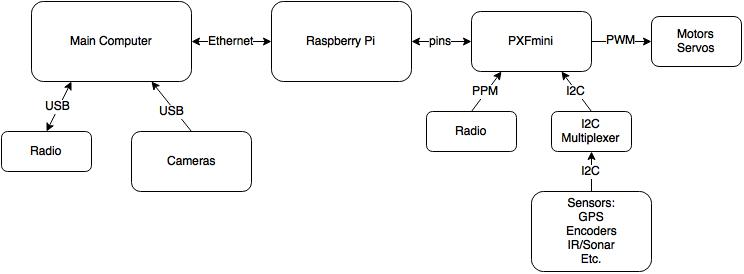
\includegraphics{Block_Diagram}
            \caption{Main Project Components}
            \label{fig:my_label}
        \end{figure}

    \subsection{Software Installation}
    \textbf{GT AutoRally Instructions}\\
    Step-by-step instructions on how to run our implementation of the GT AutoRally simulation platform.\\

    \begin{itemize}
    	\item Go to \href{https://github.com/AutoRally/autorally}{https://github.com/AutoRally/autorally} and follow the instructions to install the AutoRally platform. Be sure to follow the instructions carefully and completely, failure to do so may result in an incomplete installation that will require extended time to troubleshoot.\\
    	NOTE: It is assumed from this point on that you have already gone
through the "Autonomous Driving in Simulation" instructions at GT AutoRally.\\
    	The following instructions are intended for after completing the GT AutoRally setup and simulation instructions above.
    	\item At this point you should be able to run GT AutoRally
    	\item Keep all simulation configuration according to the AutoRally specifications.\\ e.g. stateEstimator's InvertY and InvertZ values.
    	\item Navigate to the work space where you put the AutoRally package. And then go to the src/autorally directory.
    	NOTE: All files/folders modified and provided by ARC for AutoRally are found in the arc\_autorally folder.\\
    	\item Under autorally\_description/urdf, replace the autoRallyPlatform.urdf.xacro file with file of the same name that we provide.
    	\item Copy the world folder we provide to autorally\_description/models.
    	\item Under autorally\_description, there is a file named empty\_sky\_AR.world. Copy the code below to the end of the file (before the last ""):\\ model://urdf/models/world
    	\item Under autorally\_gazebo/launch, there is a file named autoRallyTrackWorld.launch, comment out the last node (named spawn\_track).
    	\item Copy the autorally\_smartdriving folder to src/autorally.
    	\item Open a terminal, navigate to your work space. The directory that contains devel/, src/ and build/.
    	\item Use catkin\_make to compile the package.
    	\item Open the bashrc by typing in gedit ~/.bashrc.
    	\item At the bottom of the file, add these two lines: source workspace\_directory/devel/setup.bash source workspace\_directory/src/autorally/autorally\_util/setupEnvLocal.sh (Replace the workspace\_directory with your actually work space directory)
    	\item Copy the run\_autorally.sh we provide to your work space.
    	\item Open another terminal, navigate to your work space and run the run\_autorally.sh script.
    	\item run\_autorally.sh script automates the initialization processes of the GT AutoRally simulation.
    	\item A single terminal window opens opens with sub-divided windows using tmux.
    	\item Applications necessary for AutoRally will open next, including Gazebo and rqt\_publisher. These applications along with other processes are launched by the script within different tmux sub-windows in the main terminal window.
    	\item Find the application window (seperate from the terminal window) titled "rqt\_publisher".
    	\item Go to rqt\_publisher and make sure the topics created during initial setup are still there:\\ /runStop /chassisState /constantSpeedController/speedCommand
    	\item If rqt\_publisher does not have those three topics in the main part of the window, go back to the setup instructions and add them.
    	\item Make sure /runStop is set to true and speed (under /speedCommand) is set to 3. Then check the boxes to the left of those three topics.
    	\item Run these two commands in two of the tmux windows:\\ roslaunch autorally\_smartdriving autorally\_configuration.launch roslaunch autorally\_smartdriving move\_base.launch
    	\item Go back to the rqt\_publisher window and uncheck the constantspeedcontroller message.
    	\item Terminate the waypointfollower and the constantspeedcontroller.
    	\item Copy the rviz config file we provide.
    	\item roslaunch autorally\_smartdriving auto\_turn.launch
    	\item run rviz with the rviz config file. rosrun rviz rviz
    	\item Now you can set goals through Rviz and the car should go towards the goal autonomously.
    \end{itemize}
    
    \textbf{ROS Indigo Installation}\\
    If you are not installing AutoRally (which links you to the ROS installation instructions), then you will need to install ROS before doing anything else with ARC.\\
    Go to \href{http://wiki.ros.org/indigo/Installation/Ubuntu}{http://wiki.ros.org/indigo/Installation/Ubuntu} and follow the official instructions for installing ROS Indigo.

    \textbf{Stage Installation Instructions}\\
    All files modified by ARC for use in the Stage simulator are found in the arc\_stage folder provided.

    \begin{itemize}
    	\item Navigate to the work space where you put the AutoRally package. And then go to the src/autorally directory.
    	\item Copy the stage\_launch folder in arc\_stage to src/autorally.
    	\item Open a terminal, navigate to your work space. The directory that contains devel/, src/ and build/
    	\item Use catkin\_make to compile the package.
    \end{itemize}

    \subsection{Special Considerations}
    \begin{itemize}
        \item Ubuntu 14.04 was used on the primary computer and is required for the version of ROS (Indigo) that we used.
        \item ARC requires use of ROS Indigo, specifically. Newer versions of ROS might work, but have not been tested.
        \item If you go with a PXFMini, you will need to get a custom Raspberry Pi 3 image from them.
    \end{itemize}
    
    \subsection{User Guides, API documentation, Etc.} 
    \begin{itemize}
        \item MAVLink API: \href{https://github.com/mavlink}{https://github.com/mavlink}
        \item Traxxas Summit owner's manual: \href{https://traxxas.com/sites/default/files/110829-R02-5607-manual.pdf}{https://traxxas.com/sites/default/files/110829-R02-5607-manual.pdf}
        \item PXFMini documentation: \href{http://docs.erlerobotics.com/brains/pxfmini}{http://docs.erlerobotics.com/brains/pxfmini}
    \end{itemize}

\section{New Technology Learned}
\begin{itemize}
    \item \textit{What web sites were helpful?}
      \begin{itemize}
        \item \url{http://wiki.ros.org}
        \item \url{https://github.com/AutoRally/autorally}
      \end{itemize}
    \item \textit{What, if any, reference books really helped?}\par
      We did not use any reference books.
    \item \textit{Were there any people on campus that were really helpful?}\par
      Our client was Kevin, who was also our instructor. So it was very helpful.
      He provided us with all the hardware and gave us instructions on how to use them.
\end{itemize}

\section{What We Learned}
  \begin{itemize}
    \item We experienced how a research project was approximately carried out.
    \item We got to work in a diverse team, which helped us improve our
    communication skills.
    \item When working in a small team, the relationship between teammates became
    more intimate, which make us become more considerate people.
    \item ROS was a big part of this project, and we only had little to none
    experience working with. We learned a lot on how to use ROS. What we were able
    to accomplish was incredible.
    \item MORE TO ADD.
  \end{itemize}

\subsection{Cierra}
\begin{itemize}
    \item What technical information did you learn?
    \item What non-technical information did you learn?
    \item What have you learned about project work?
    \item What have you learned about project management?
    \item What have you learned about working in teams?
    \item If you could do it all over, what would you do differently?
\end{itemize}

\subsection{Tao}
\begin{itemize}
    \item What technical information did you learn?
    \begin{itemize}
      \item A basic structure of a project.
      \item Using ROS.
      \item Version control.
    \end{itemize}
    \item What non-technical information did you learn?
    \begin{itemize}
      \item Communicating with teammates.
      \item Explaining concepts and reporting to client.
      \item Recording progress.
      \item For me personally, this project made me like to think about
      problems with the big picture while focusing on the individual components.
    \end{itemize}
    \item What have you learned about project work?
    \begin{itemize}
      \item Coding could be easy if the project was planed out nicely.
      \item To make a good plan, one must view the project from different
      prospectives, and listen to others' opinions.
      \item Keeping track of progress is extremely important.
      \item Stick with the plan, and yet quickly switch other solutions
      when the original does not work out.
    \end{itemize}
    \item What have you learned about project management?
      \begin{itemize}
        \item Lists are useful for keeping track of hardware.
        \item Version control is important but be careful when using it.
      \end{itemize}
    \item What have you learned about working in teams?
    \begin{itemize}
      \item Good teammates are key. It depends on luck.
      \item Always try to create a positive atmosphere even things aren't
      working so well.
      \item Helping teammates out is not sacrificing. You gain more than you
      lose.
    \end{itemize}
    \item If you could do it all over, what would you do differently?
    \begin{itemize}
      \item I'd probably prioritize things differently and look for other options
      when something didn't work out. For example, we could have worked on the
      software and hardware simultaneously, which I think was our original plan.
      But then we hit a road block that totally stalled our work on hardware from
      progressing. Other than that, I don't think I would do much different.
    \end{itemize}
\end{itemize}

\subsection{Dan}
\begin{itemize}

    \item What technical information did you learn?
    \begin{itemize}
        \item How to develop for robots:\\
        The Robotics Operating System (ROS) is an open source general-purpose software
        platform for developers working with all manner of robots. ROS allows the developer to 
        use its extensive libraries to implement custom code for controlling robots and provides communications and navigation libraries that are very useful for autonomous vehicle applications. We wrote some programs in C and python using Ros libraries to communicate with the vehicle.
        \item How to set up simulators:\\
        I used both Gazebo and Stage are simulation environments that we used on this project. I learned how to set up and run both.
        \item RC cars and Autonomy\\
        I had never worked with RC cars, or tried any sort of robotics, so diving into the field of autonomous vehicles really stretched me. There is \textit{so much} that goes into research and development of autonomous vehicles. The computer has to either know the exact state of the vehicle via sensor data, or be able to estimate the vehicle's state closely enough to operate.
        \item \href{https:\\cmake.org}{CMake}\\
        CMake is a platform for build and testing software. It is open source. ROS uses CMake as part of its package installation platform, called Catkin.        
        \item I learned more about bash and Linux, creating a script to launch AutoRally, spawning multiple terminals and processes.
        \item I learned about lidar and point-clouds. I had never seen lidar in action before. I learned that there are different types of lidar. We used IR and some sort of LED technology.
    \end{itemize}
    
    \item What non-technical information did you learn?
    \begin{itemize}
        \item I learned that "autonomous" has many different meanings when related to vehicles. My assumption was that it meant that cars could navigate pretty much anywhere on their own. I found out that a car can be considered "autonomous" if it performs \textit{any} operation on its own. For instance, Georgia Tech's AutoRally project claims their car is "autonomous" and the car does go around a track without a user controlling the car directly. However, the car does guide itself, it follows predetermined way-points and performs no obstacle avoidance what-so-ever. The barriers around the track were in place to merely keep the car from going completely off the rails should something go wrong. The car did self-correct steering around the turns and kept the car under control will power-sliding around corners. So, the car was autonomous, just not in the way that I had though.
    \end{itemize}
    
    \item What have you learned about project work?
    \begin{itemize}
        \item Plan for setbacks and do not be disappointed when they happen.
        \item It's really hard to work on a complicated project part time while taking other classes.
        \item Ten hours of trial and error will save an hour of good design planning.
        \end{itemize}
    
    \item What have you learned about project management?
        \begin{itemize}
        \item It would be very helpful to use project management software.
        \subitem My team did \textit{not} use any sort of project management software for this project, by "project management software" I mean packages such as MS Project, or Redmine. Project tracking using manually implemented Gantt charts was incredibly tedious and not really used as a practical tool.
        \item Milestones need to be clearly identified and consistently communicated throughout the life of the project.
    \end{itemize}
    
    \item What have you learned about working in teams?
        \begin{itemize}
        \item I was the team leader. It was difficult to balance keeping the team focused on our goal and not squashing enthusiasm when attempting to redirect tangent ideas back on track.
        \item Good communication is key to keeping a team operating smoothly.
        \item When everyone pitches in and they are enthusiastic about the project, the work is quite fun.
    \end{itemize}
    
    \item If you could do it all over, what would you do differently?
    \begin{itemize}
        \item Identify critical points of failure. Things that could possibly set us back significantly if they were to fail.
        \subitem Test those points early, if possible.
        \item Be more proactive about getting help for problems. Don't struggle with a problem for more than a few days before getting help. 
        \item Start with a rover that has an autopilot integrated into it, possibly even already has some sensors on it.
        \subitem Our team had \textit{no} experience going into this project. Trying to start from scratch was probably a bit too much, if the goal was to implement high-speed performance. It would have been more realistic to attain if we had started with a vehicle that had some sort of autonomous capability already and then we "upgrade" it to perform at a high rate of speed.
        \item I would use project management software.
        \item I would set an expectation of a required weekly meeting time at the beginning of the project. Our team agreed to do that, but I did not really follow through on it well.
    \end{itemize}
\end{itemize}

\section{Appendix 1}
Essential Code Listings. You don't have to include absolutely everything, but if someone wants to understand your project, there should be enough here to learn from. If you worked within a larger project, something like a patch file might be a good way to go.
\begin{lstlisting}[frame=single,caption={Example Custom ROS Node}]
/**********************************************
* @file lidarDetection.cpp
* @author Tao Chen <chentao@oregonstate.edu>
* @date Feburary 21, 2017
* @copyright 2017 Oregon State University
* @brief ROS node to generate new waypoints based on lidar scan
*
* @details When an obstacle is detected, it alters the original
* set of waypoints to go around the obstacle. This node subscribes to
* the laser_scan message and the current_list_of_waypoints message and
* publish the new_waypoints message.
***********************************************/

#include "lidarDetection.h"

namespace autorally_smartdriving{
	LidarDetection::LidarDetection(){
		l_lidarSub = l_nh.subscribe("/autorally_platform/laser_scan", 10, &LidarDetection::gatherLidarData, this);
		l_lidarPub = l_nh.advertise<sensor_msgs::LaserScan>("scan", 10);

		samples = 2000;
		laser_frequency = 10;
		scan.ranges.resize(samples);
		scan.intensities.resize(samples);
	}

	LidarDetection::~LidarDetection(){}

	void LidarDetection::gatherLidarData(sensor_msgs::LaserScan data){
		int counter = 0;

		ros::Time scan_time = ros::Time::now();

		scan.header.stamp = scan_time;
		scan.header.frame_id = "lidar";
		scan.angle_min = data.angle_min;
		scan.angle_max = data.angle_max;
		scan.angle_increment = data.angle_max / samples;
		scan.time_increment = (1 / laser_frequency) / samples;
		scan.range_min = data.range_min;
		scan.range_max = data.range_max;

		for(counter = 0; counter < samples; counter++){
			scan.ranges[counter] = data.ranges[counter];
			scan.intensities[counter] = data.intensities[counter];
		}

		// publish scan to scan topic
		l_lidarPub.publish(scan);
	}
};

int main(int argc, char** argv){
	ros::init(argc, argv, "LidarDetection");
	autorally_smartdriving::LidarDetection lidarDetection;
	ros::spin();
}
\end{lstlisting}

\begin{lstlisting}[frame=single,caption={Example Custom Launch File for Stage}]
<launch>

  <!--  ************** Global Parameters ***************  -->
  <param name="/use_sim_time" value="true"/>

  <!--  ************** Stage Simulator ***************  -->
  <node pkg="stage_ros" type="stageros" name="stageros" args="$(find stage_launch)/stage/empty.world">
    <!-- <remap from="base_scan" to="scan"/> -->
    <remap from="base_scan" to="base_scan_0"/>
  </node>

  <node pkg="move_base" type="move_base" respawn="false" name="move_base" output="screen">
    <rosparam file="$(find smart_driving)/config/costmap_common_params.yaml" command="load" ns="global_costmap" />
    <rosparam file="$(find smart_driving)/config/costmap_common_params.yaml" command="load" ns="local_costmap" />
    <rosparam file="$(find smart_driving)/config/local_costmap_params.yaml" command="load" />
    <rosparam file="$(find smart_driving)/config/global_costmap_params.yaml" command="load" />
    <rosparam file="$(find smart_driving)/config/base_local_planner_params.yaml" command="load" />

    <param name="base_global_planner" value="global_planner/GlobalPlanner" />
    <param name="planner_frequency" value="1.0" />
    <param name="planner_patience" value="5.0" />

    <param name="base_local_planner" value="teb_local_planner/TebLocalPlannerROS" />
    <param name="controller_frequency" value="5.0" />
    <param name="controller_patience" value="15.0" />

    <param name="clearing_rotation_allowed" value="false" />
  </node>

  <node name="map_server" pkg="map_server" type="map_server" args="$(find stage_launch)/maps/empty_world.yaml" output="screen">
    <param name="frame_id" value="/map" />
  </node>

  <!--<node pkg="amcl" type="amcl" name="amcl" output="screen">
    <rosparam file="$(find stage_launch)/cfg/amcl_params.yaml" command="load"/>
    <param name="initial_pose_x" value="0" />
    <param name="initial_pose_y" value="0" />
    <param name="initial_pose_z" value="0" />
  </ode>-->

  <!-- <include file="$(find leddar)/launch/leddar.launch">
    <arg name="serial" value="AJ04071" />
    <arg name="frame" value="base_laser_link_0" />
    <arg name="fov" value="45" />
    <arg name="range" value="50" />
  </include> -->

  <include file="$(find stage_launch)/robot_localization.launch"/>

  <node name="odom" pkg="autorally_smartdriving" type="odom" />
  <node name="rviz" pkg="rviz" type="rviz" args="-d $(find stage_launch)/stage/rviz_navigation.rviz"/>
</launch>
\end{lstlisting}

\section{Appendix 2}
Anything else you want to include. Photos, etc.

\end{document}

